%TODO: PONER IMAGENES DE EJEMPLO DE LOS FICHEROS DEL EJERCICIO 1
%TODO 2: INTENTAR QUITAR LA MORRAYA QUE NO SIRVA
%TODO 3: INTENTAR NO REPETIR TANTAS COSAS EN EL EJERCICIO 3
\documentclass{article}
\usepackage[utf8]{inputenc}
\usepackage[spanish]{babel}
\usepackage{graphicx, graphics, float, hyperref}
\usepackage{listings}
\usepackage[a4paper, total={6in, 10in}]{geometry}

\title{SSO Práctica 1}
\author{Andrés Merlo Trujillo}
\date{}
\hypersetup{
    colorlinks=true,
    linkcolor=black,
}

\begin{document}

\maketitle

\tableofcontents

\section{Primer ejercicio}
A continuación, voy a explicar el formato y el significado de cada uno de los campos. Para ello, voy a dividir cada archivo en subsecciones:

\subsection{/etc/passwd}
\textbf{Formato:} \verb|nombre_login:contra_encriptada:UID:GID:comentario:shell|

\begin{figure}[H]
    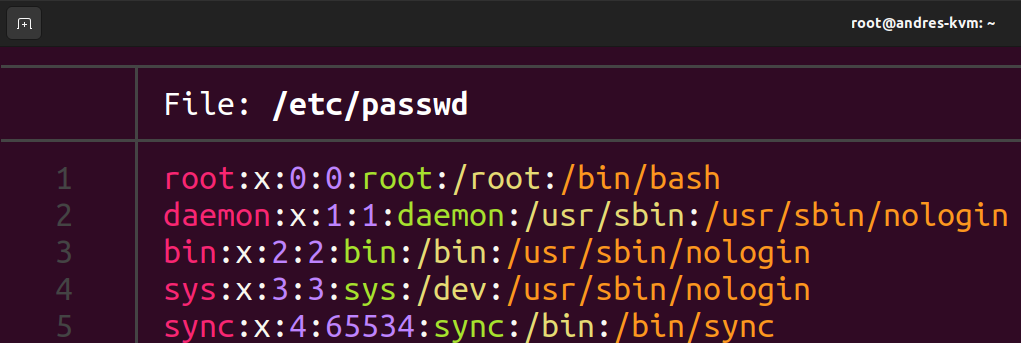
\includegraphics[width=\textwidth]{imagenes/passwdfile.png}
    \caption{Ejemplo de entradas en el archivo.}
\end{figure}

\bigskip

Este fichero está formado por líneas de 7 campos separados por ``:''. Los campos y sus significados son los siguientes:

\begin{enumerate}
    \item \textbf{Nombre de login: }Nombre de usuario.
    \item \textbf{Contraseña encriptada opcional: }Contraseña encriptada del usuario.
    Si este campo tiene la letra ``x'' minuscula, significa que la contraseña se almacena en ``/etc/shadow''.

    Si se encuentra vacio, significa que no hace falta contraseña para autenticar.

    Si comienza en exclamacion, significa que la contraseña ha sido bloqueada.

    Ademas, si contiene una exclamacion o un asterisco, significa que el usuario no podra usar la contraseña para iniciar sesion (pero puede usar otro medio).

    \item \textbf{User ID numerico: }ID del usuario.
    \item \textbf{Group ID numerico: }ID del grupo al que pertenece.
    \item \textbf{Nombre de usuario o campo de comentario: }Este campo sirve para poder poner un comentario sobre el usuario (por ejemplo: accion que realiza, para evitar confusion con dos usuarios similares, etc).
    \item \textbf{Directorio home del usuario: }Directorio que será el home privado del usuario. Además sirve para poner la variable de entorno ``\$HOME''
    \item \textbf{Interprete opcional de comando de usuario: }Shell que usará el usuario por defecto (bash, sh, zsh, fish, etc). Ademas, pondra la variable de entorno ``\$SHELL'' a este valor.
\end{enumerate}


\subsection{/etc/group}
\textbf{Formato: }\verb|nombre_grupo:contra:GID:usuario1,usuario2,...|

\begin{figure}[H]
    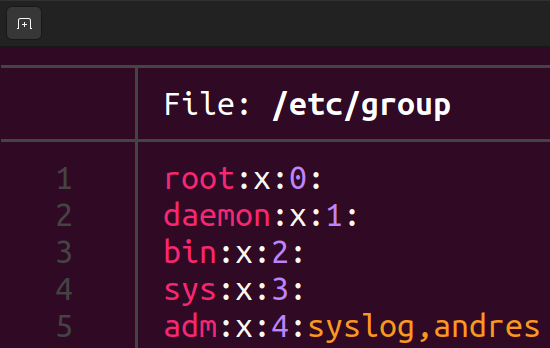
\includegraphics[width=\textwidth]{imagenes/groupfile.png}
    \caption{Ejemplo de entradas en el archivo.}    
\end{figure}

\bigskip

Este fichero está formado por 4 campos separados por ``:''. EL significado de cada campo es el siguiente:

\begin{enumerate}
    \item \textbf{Nombre del grupo: }Nombre del grupo. Este nombre debe ser único en el sistema.
    
    %REVISAR ESTE CAMPO
    \item \textbf{Contraseña: }Contraseña del grupo. Si es una letra ``x'' minuscula significa que la contraseña encriptada se encuentra en ``/etc/gpasswd''.
    \item \textbf{Group ID: }Indica el ID del grupo. Este valor debe ser único en el sistema.
    \item \textbf{Usuarios: }Lista de ususarios separados por coma (``,'') los cuales son miembros del grupo. 
\end{enumerate}
\subsection{/etc/shadow}
\textbf{Formato: }\verb|login:pass:last_change:min_age:max_age:pass_warn:pass_inact:acc_exp:reserved|

\begin{figure}[H]
    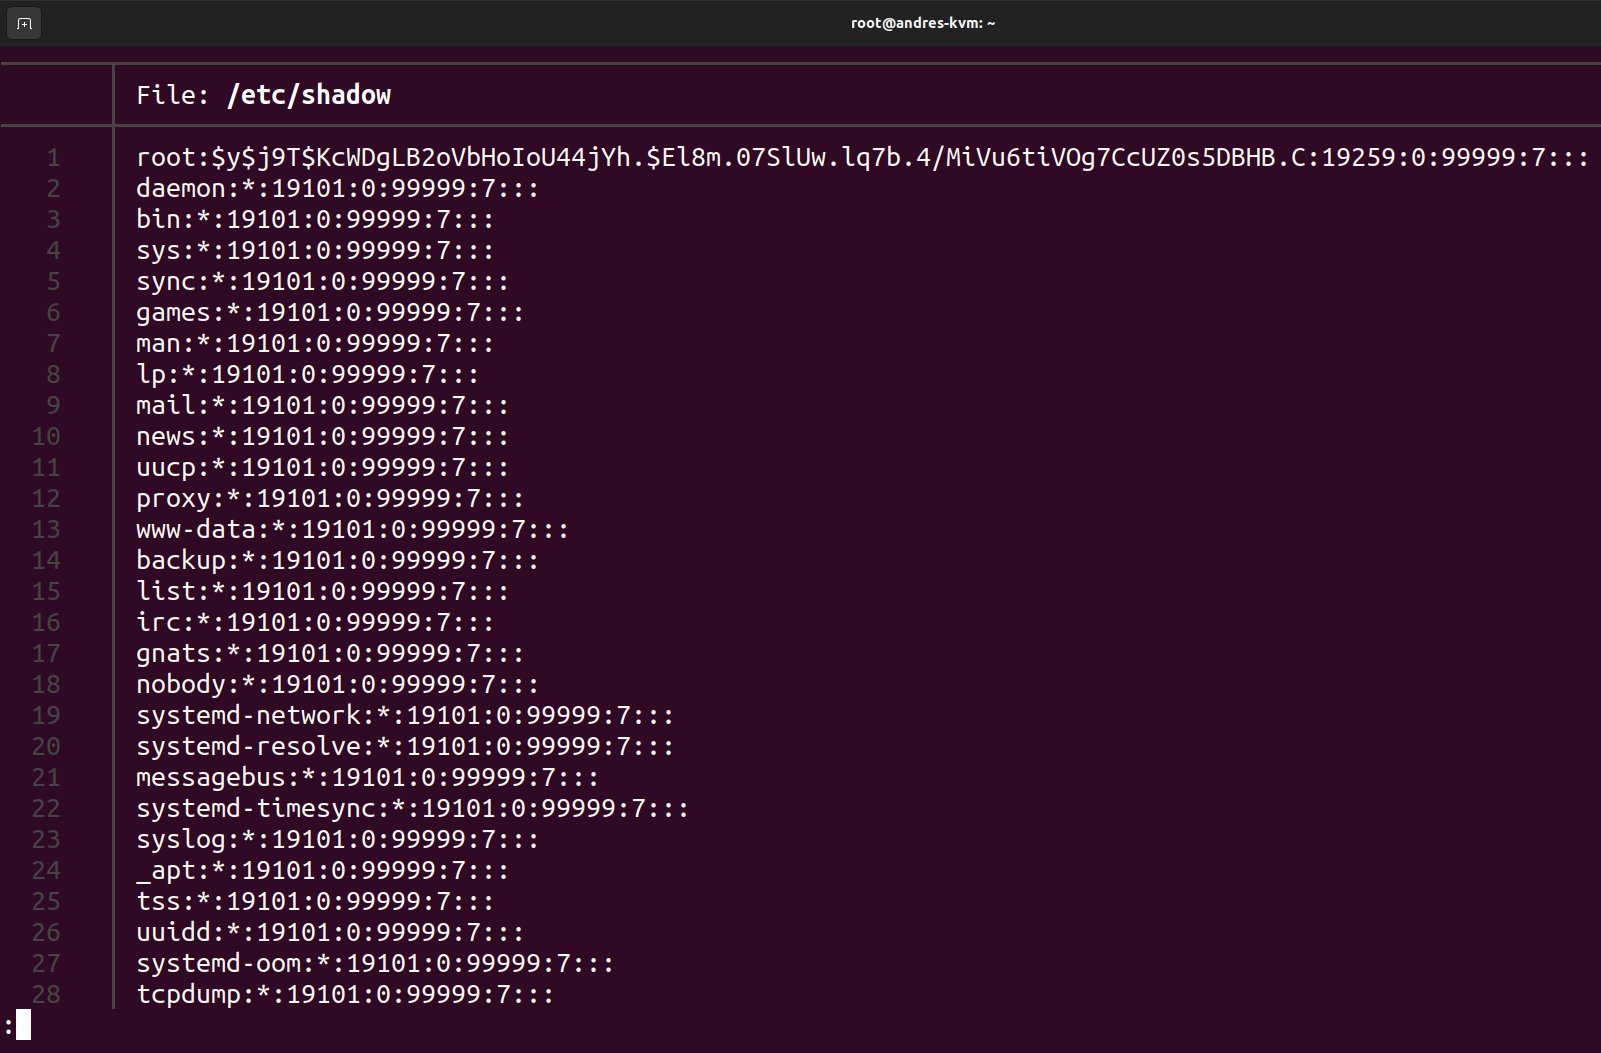
\includegraphics[width=\textwidth]{imagenes/shadowfile.png}
    \caption{Ejemplo de entradas en el archivo.}    
\end{figure}

\bigskip

Este fichero está formado por líneas de 9 campos separados por ``:''. Los campos y sus significados son los siguientes:

\begin{enumerate}
    \item \textbf{login name (nombre de login): }Nombre de la cuenta del usuario. Debe existir en el sistema.
    
    %Hablar de la encriptacion concreta que tiene (quizas sea un salteo)
    \item \textbf{encrypted password (contraseña encryptada): }Contraseña encriptada del usuario especificado en ``login name''. Si este campo está vacío, significa que ese usuario no requiere contraseña para iniciar sesion. 
    
    Además, en caso de que la contraseña comience con una exclamacion (``!''), significa que la contraseña ha sido bloqueada.

    Por último, si la contraseña contiene el carácter de exclamacion mencionado anteriormente o asterisco (``*''), significa que no puede iniciar sesión (si es exclamación también se cumple lo de arriba).

    \item \textbf{date of last password change (fecha del ultimo cambio de contraseña): }El último cambio de contraseña, expresado como el numero de dias desde el epoch (1 de enero de 1970).
    
    Además, si el valor es 0 significa que el usuario debe cambiar la contraseña en el proximo login.

    %comprobar este parrafo
    En cambio, si el campo está vacio signicia que las contraseñas no tienen edad (y por tanto no se cumplen estas restricciones).

    \item \textbf{minimum password age (edad minima de la contraseña): }Numero de dias que el usuario tiene que esperar antes de poder cambiar la contraseña de nuevo. Un valor 0 ó vacio indica que no hay un minimo de dias.
    \item \textbf{maximum password age (edad maxima de la contraseña): }Numero maximo de dias en los cuales la contraseña ``caduca'' (tiene que cambiarla). Al pasar este numero de dias, el sistema pedira al usuario que cambie la contraseña.
    
    Si el valor maximo es mayor que el del campo anterior, el usuario no podra cambiar su contraseña.

    Por último, si el campo está vacio, se deshabilitara este servicio junto con ``password warning period'' y ``password inactivity period''.

    \item \textbf{password warning period (periodo de advertencia de la contraseña): }El numero de dias antes de que la contraseña ``caduqeu'' durante los cuales se le  advierte al usuario.
    
    Un valor 0 o cadena vacia indica que no habra advertencias.

    \item \textbf{password inactivity period (periodo de inactividad de la contraseña): }Numero de dias despues de que la contraseña haya ``caducado'' en el cual eberia ser aceptada. Al pasar este eriodo, el usuario no podra iniciar sesion.
    
    Un campo vacio indica que no se cumple esta regla.

    \item  \textbf{account expiration date (fecha de expiracion de la cuenta): }La fecha en la que la cuenta expira. Esta fecha se exresa como el numero de dias desde el epoch.
    
    La diferencia con la expiracion de una contraseña es que, si la cuenta expira, no podra iniciar sesion de ninguna forma, mientras que si la contraseña expira, tendrá otros medios para iniciar sesion.

    El campo vacio indica que la cuenta no expira. Ademas, no se debe usar el valor 0 ya que se puede interpretar como que la cuenta expira en el epoch o que no expira.

    \item \textbf{reserved field (campo reservado): }Este campo está reservado para usos futuros.
\end{enumerate}

\subsection{/etc/gshadow}
\textbf{Formato: }\verb|group_name:encrypted_pass:admin1,admin2,...:member1,member2,...|

\bigskip

\begin{figure}[H]
    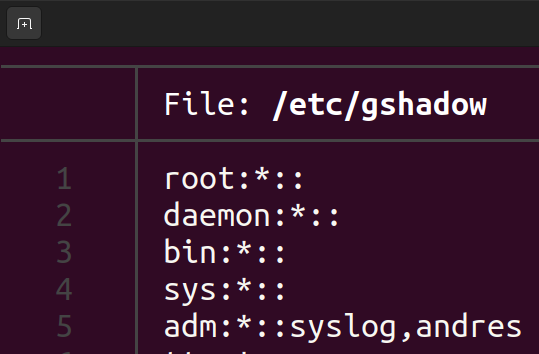
\includegraphics[width=\textwidth]{imagenes/gshadowfile.png}
    \caption{Ejemplo de entradas en el archivo.}    
\end{figure}

Este fichero está tambien formado por 4 campos separados por el símbolo ``:''. El significado de cada campo es el siguiente:

\begin{enumerate}
    \item \textbf{Nombre del grupo: }Nombre del grupo. Debe existir en el sistema.
    \item \textbf{Contraseña encriptada: }Contraseña encriptada que sirve para que un usuario que no es miembro del grupo obtenga los permisos.
    
    Si el campo está vacio, entonces cualquier usuario puede obtener los privilegios del grupo.

    Si la contraseña comienza por una exclamacion, significa que esta está bloqueada.

    Si contiene una exclamacion o asterisco, los usuarios no podran acceder al grupo si no estan en el.

    \item \textbf{Administradores: }Lista de usuarios separados por coma que puede realizar operaciones como cambiar la contrasñéa del grupo o administrar los usuarios del mismo.
    \item \textbf{Miembros: }Lista de usaurios separados por coma. Los miembros del grupo pueden acceder al mismo sin necesitar la contraseña.
\end{enumerate}

\section{Segundo ejercicio}
En este ejercicio se pide modificar el valor de la variable ``LOGIN\_TIMEOUT'' y comprobar sus efectos con un usuario nuevo que se haya creado manualmente.

Para ello, modifico la variable, que estaba por defecto a 60 segundos:

\begin{figure}[H]
    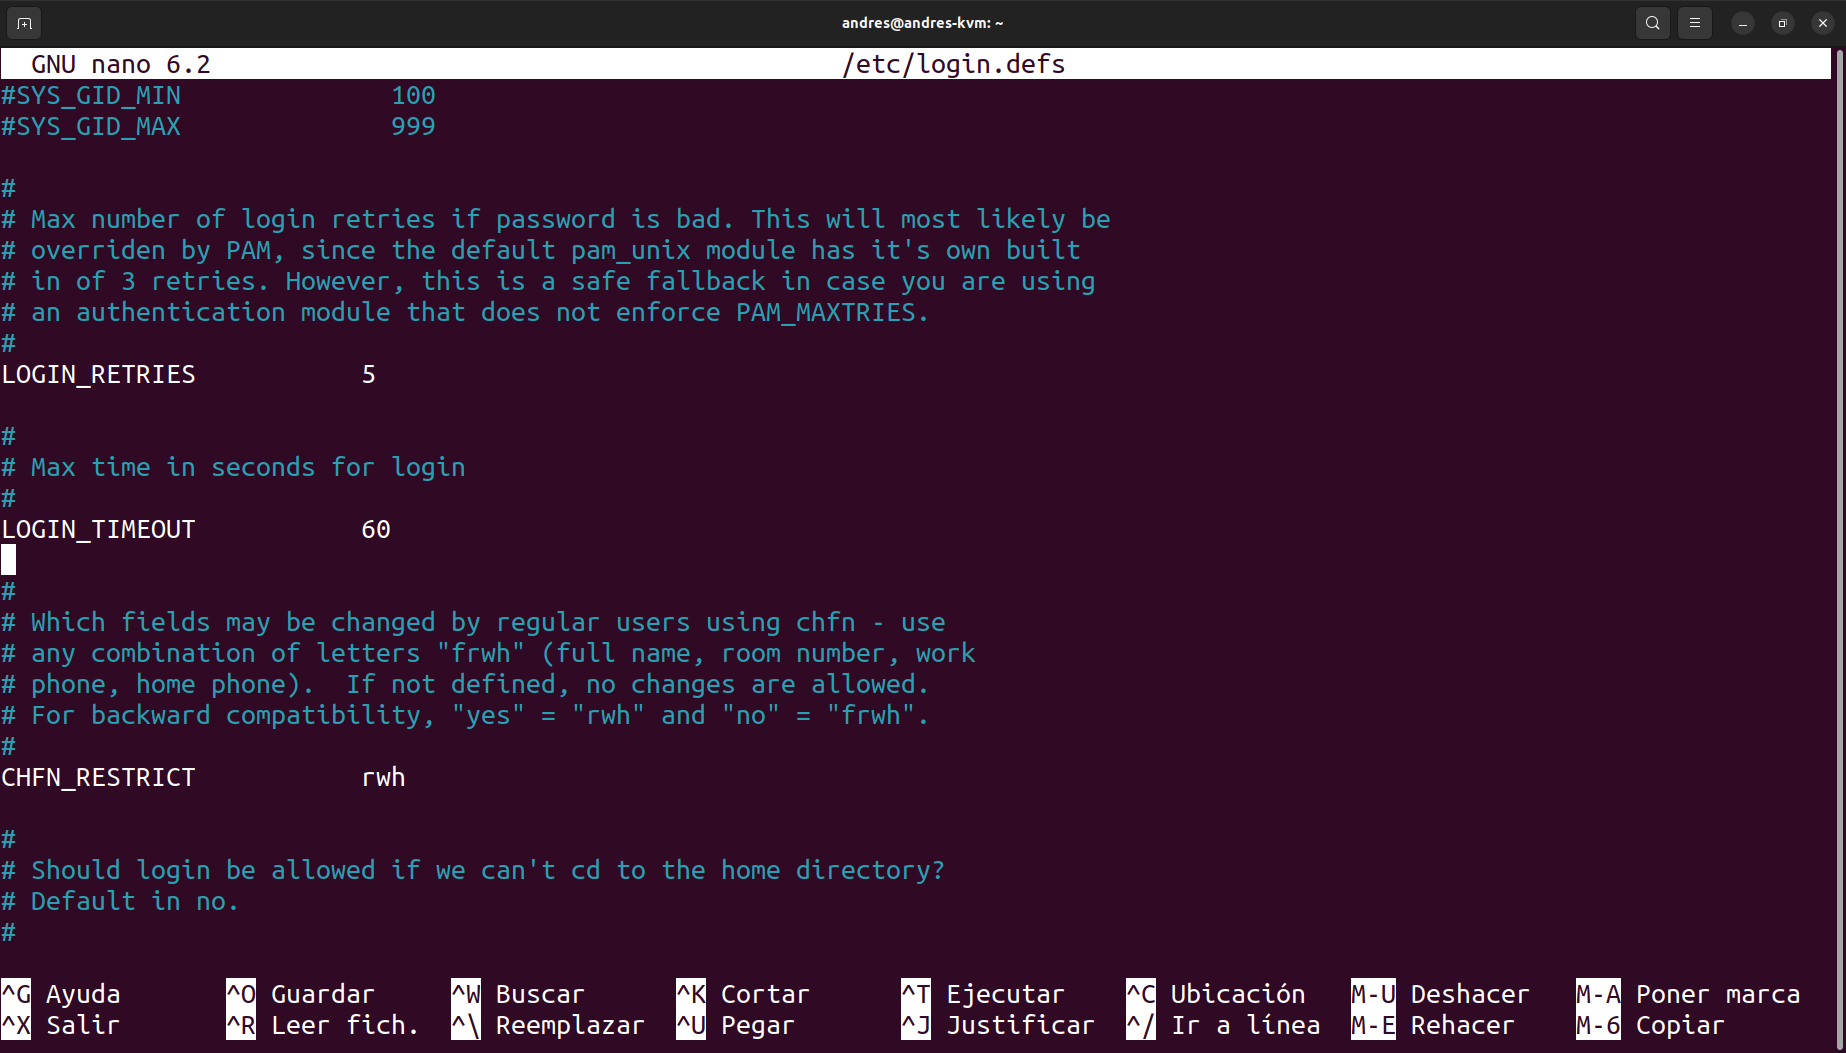
\includegraphics[width=\textwidth]{imagenes/tout60.png}
    \caption{Valor por defecto.}
\end{figure}

Y lo cambio a otro valor, por ejemplo, 5 segundos:

\begin{figure}[H]
    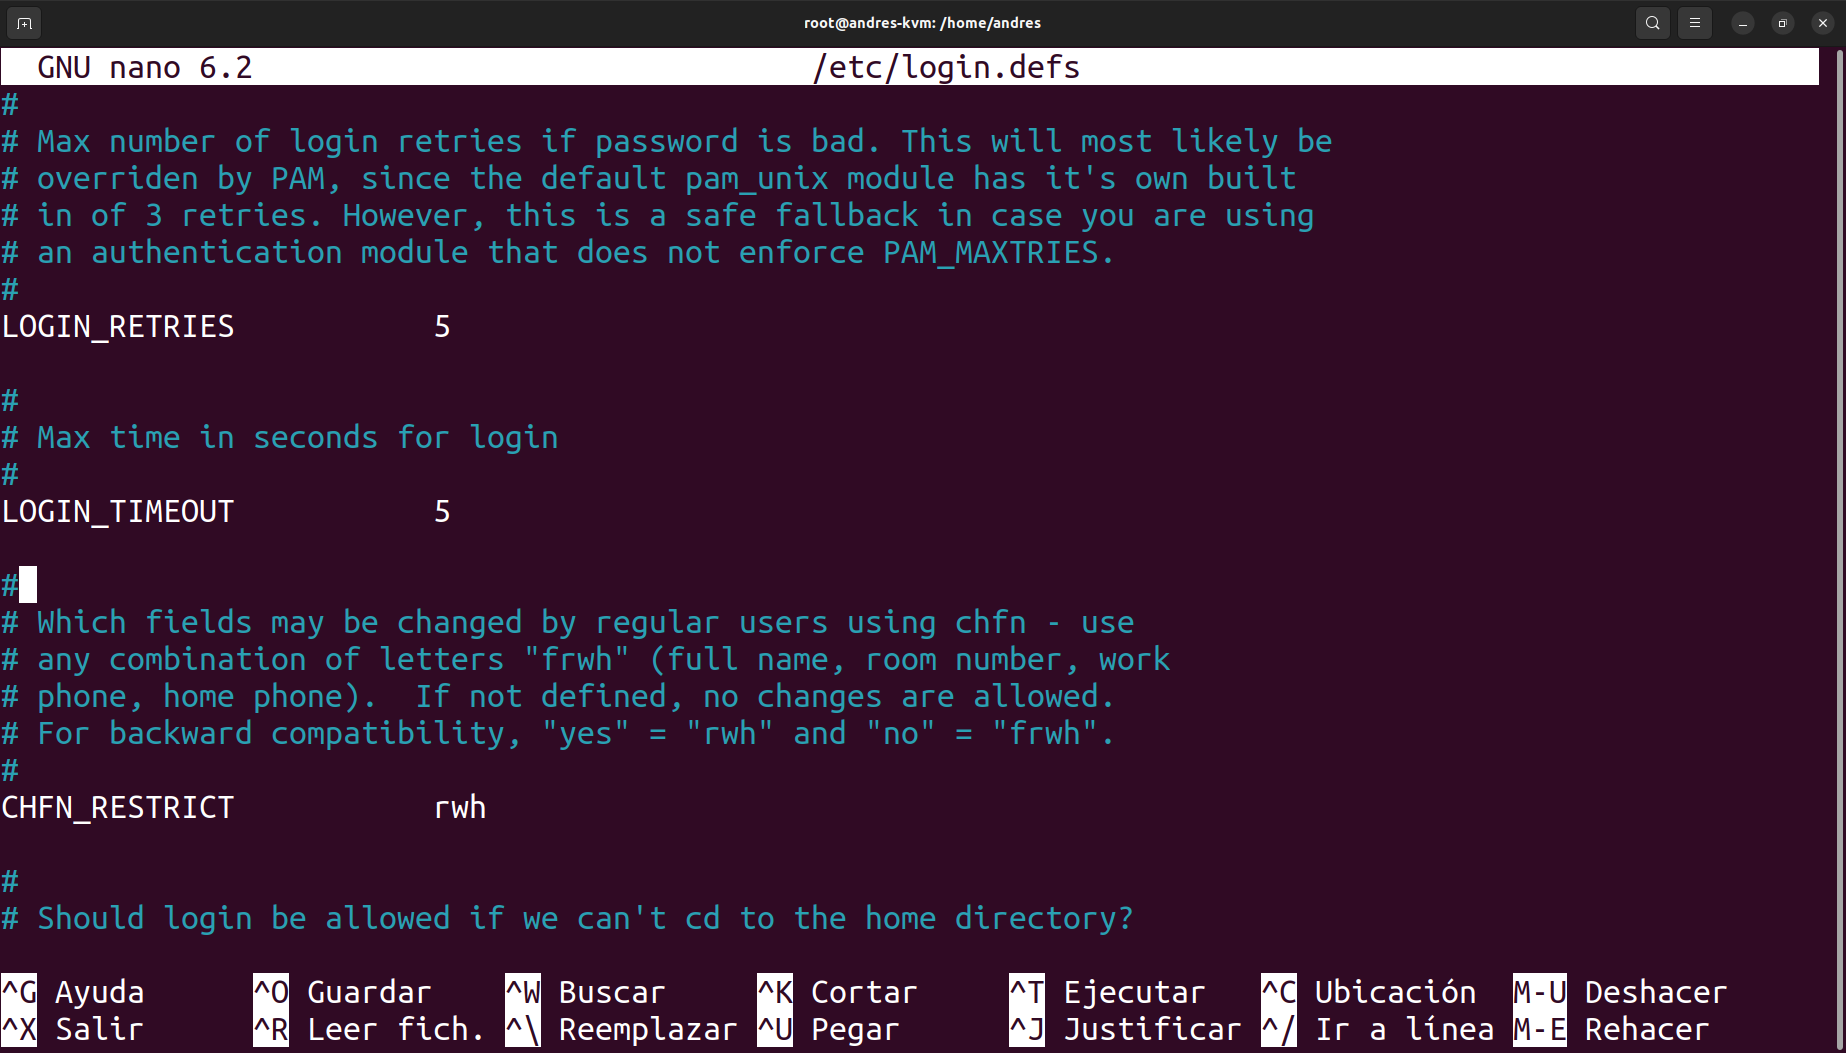
\includegraphics[width=\textwidth]{imagenes/tout5.png}
    \caption{Valor cambiado a 5 segundos.}
\end{figure}

A continuacion, creo el usuario llamado ``prueba'', le cambio la contraseña y hago login con él desde la terminal. Cuando se encuentre en la parte de pedir la contraseña de este usuario nuevo, se espera un tiempo hasta que la terminal devuevla un mensaje:

\begin{figure}[H]
    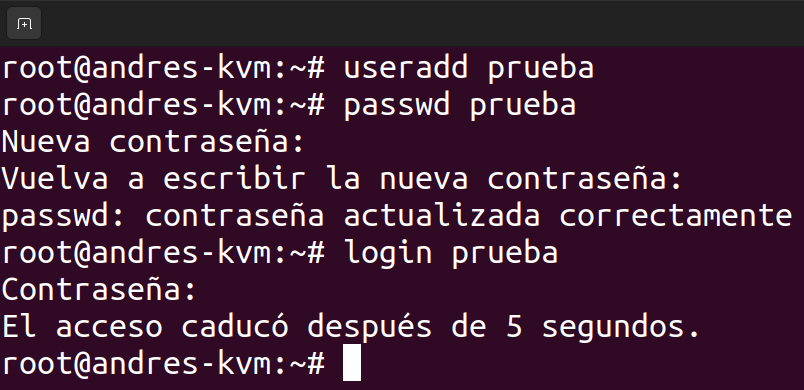
\includegraphics[width=\textwidth]{imagenes/tout5login.png}
\end{figure}

Como se puede ver, pone que han pasado 5 segundos y el acceso ha caducado.

Ahora, pruebo con otro valor, por ejemplo \textbf{12} segundos:

\begin{figure}[H]
    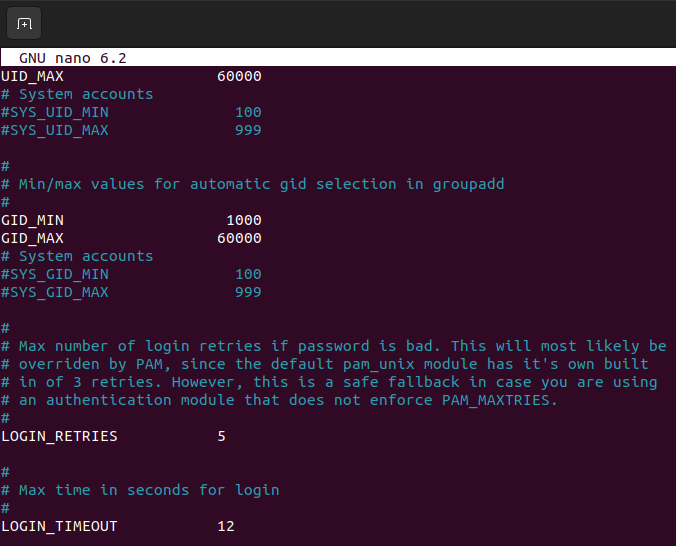
\includegraphics[width=\textwidth]{imagenes/tout12.png}
\end{figure}

E intento iniciar sesion de nueov con el usuario ``prueba'' y espero en la parte de la contraseña.

\begin{figure}[H]
    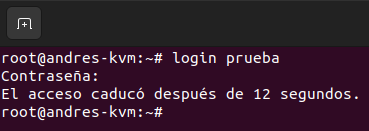
\includegraphics[width=\textwidth]{imagenes/tout12login.png}
\end{figure}

Como se puede ver, el timeout ahora es distinto.


\section{Tercer ejercicio}
En este ejercicio se pide crear un archivo y darle, mediante un ACL, permisos de lectura y escritura al usuario creado (en mi caso sigue siendo ``prueba'').

Para ello, mediante la orden ``touch'' creo el archivo denominado ``ejercicio3''.

Ahora bien, al menos en Ubuntu 22.04 no están las ordenes ``getacl/setacl'', sino que se llaman ``getfacl/setfacl''. El resultado no varía y tienen las mismas sintaxis.

\begin{figure}[H]
    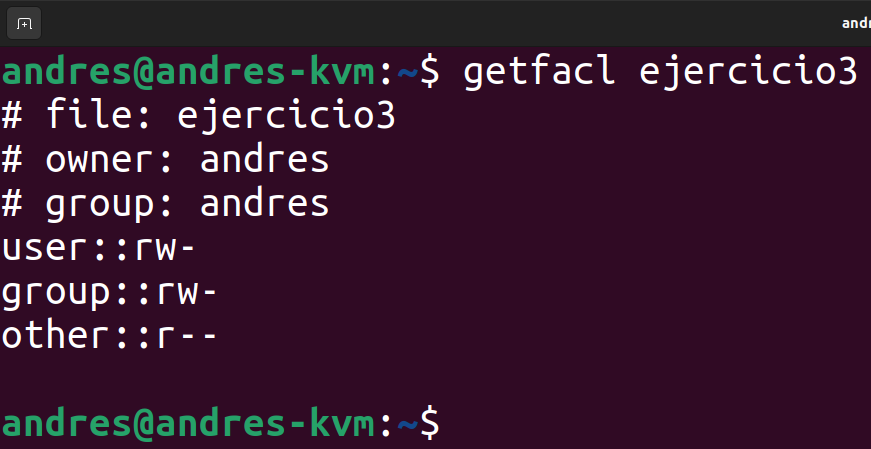
\includegraphics[width=\textwidth]{imagenes/getfaclorg.png}
    \caption{se puede ver que solo el usuario ``andres'' tiene los permisos}
\end{figure}


Ahora, con la orden \verb|setfacl -m u:prueba:rw ejercicio3| se le dará al usuario ``prueba'' permisos ``rw''. Y de nuevo mostramos con ``getfacl'' el archivo anterior:

\begin{figure}[H]
    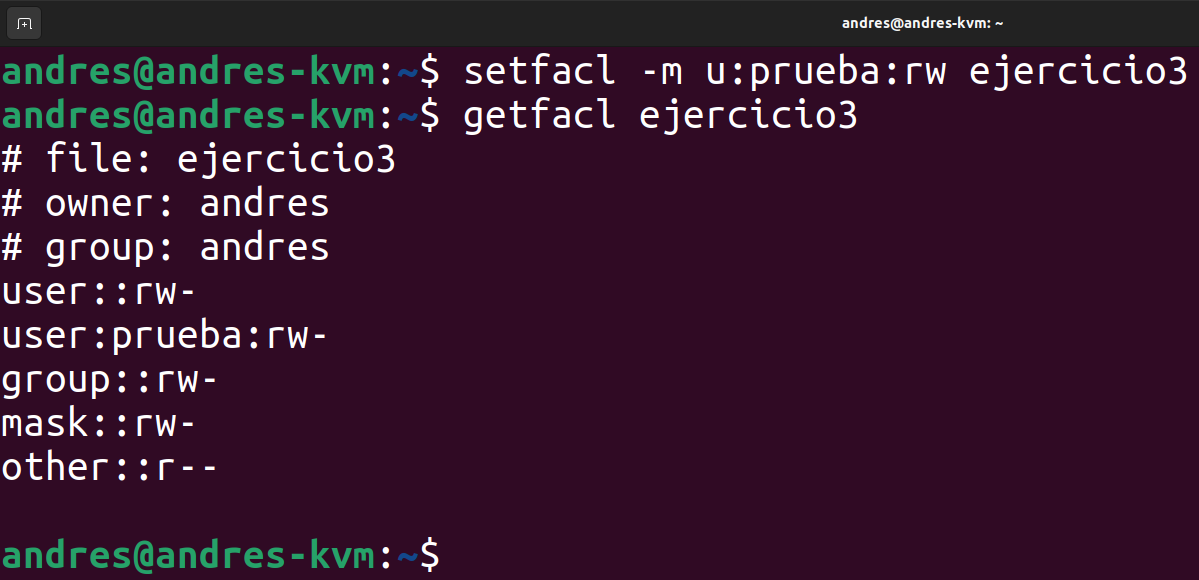
\includegraphics[width=\textwidth]{imagenes/getfaclnew.png}
    \caption{se puede ver que solo el usuario ``andres'' tiene los permisos}
\end{figure}

Como se puede observar, ahora aparece una linea que indica que el usuario ``prueba'' tiene permisos ``rw''.


\section{Ejercicio 4}
Con el comando ``ls'' muestro los archivos que se encuentran en el directorio ``/etc/pam.d'':

\begin{figure}[H]
    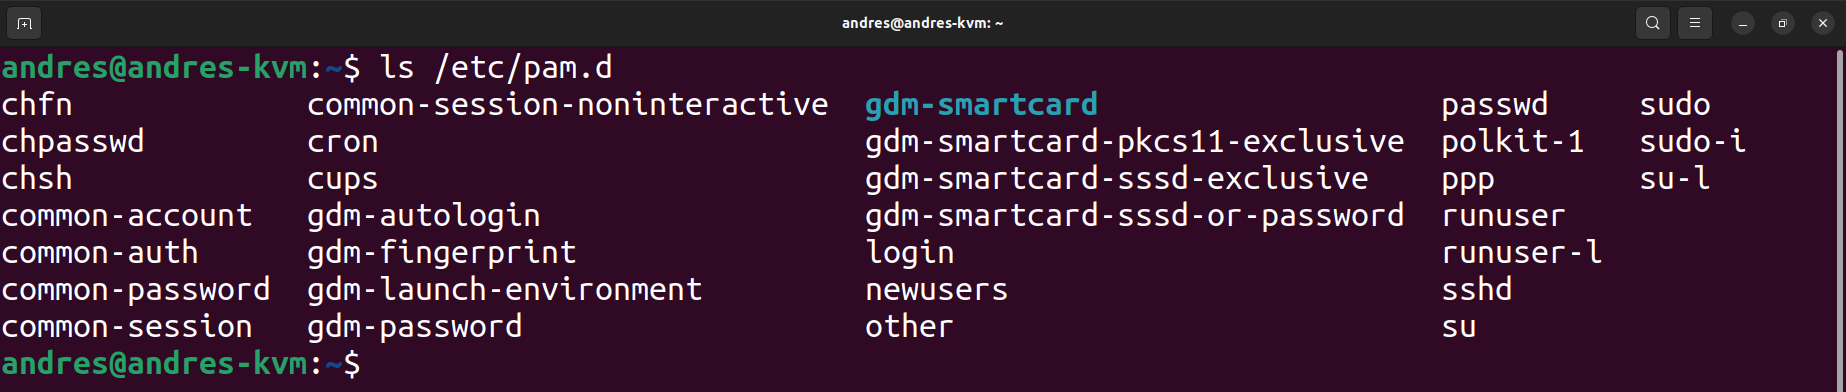
\includegraphics[width=\textwidth]{imagenes/lspam.png}
\end{figure}

A continuacion explicare dos archivos:

\subsection{/etc/pam.d/chfn}
Permite cambiar la informacion personal de un usuario tales como: el nombre, el numero de telefono, de habitacion, etc. Estos datos luego pueden ser leidos por comandos como ``finger''.

El contenido del archivo es:

\begin{figure}[H]
    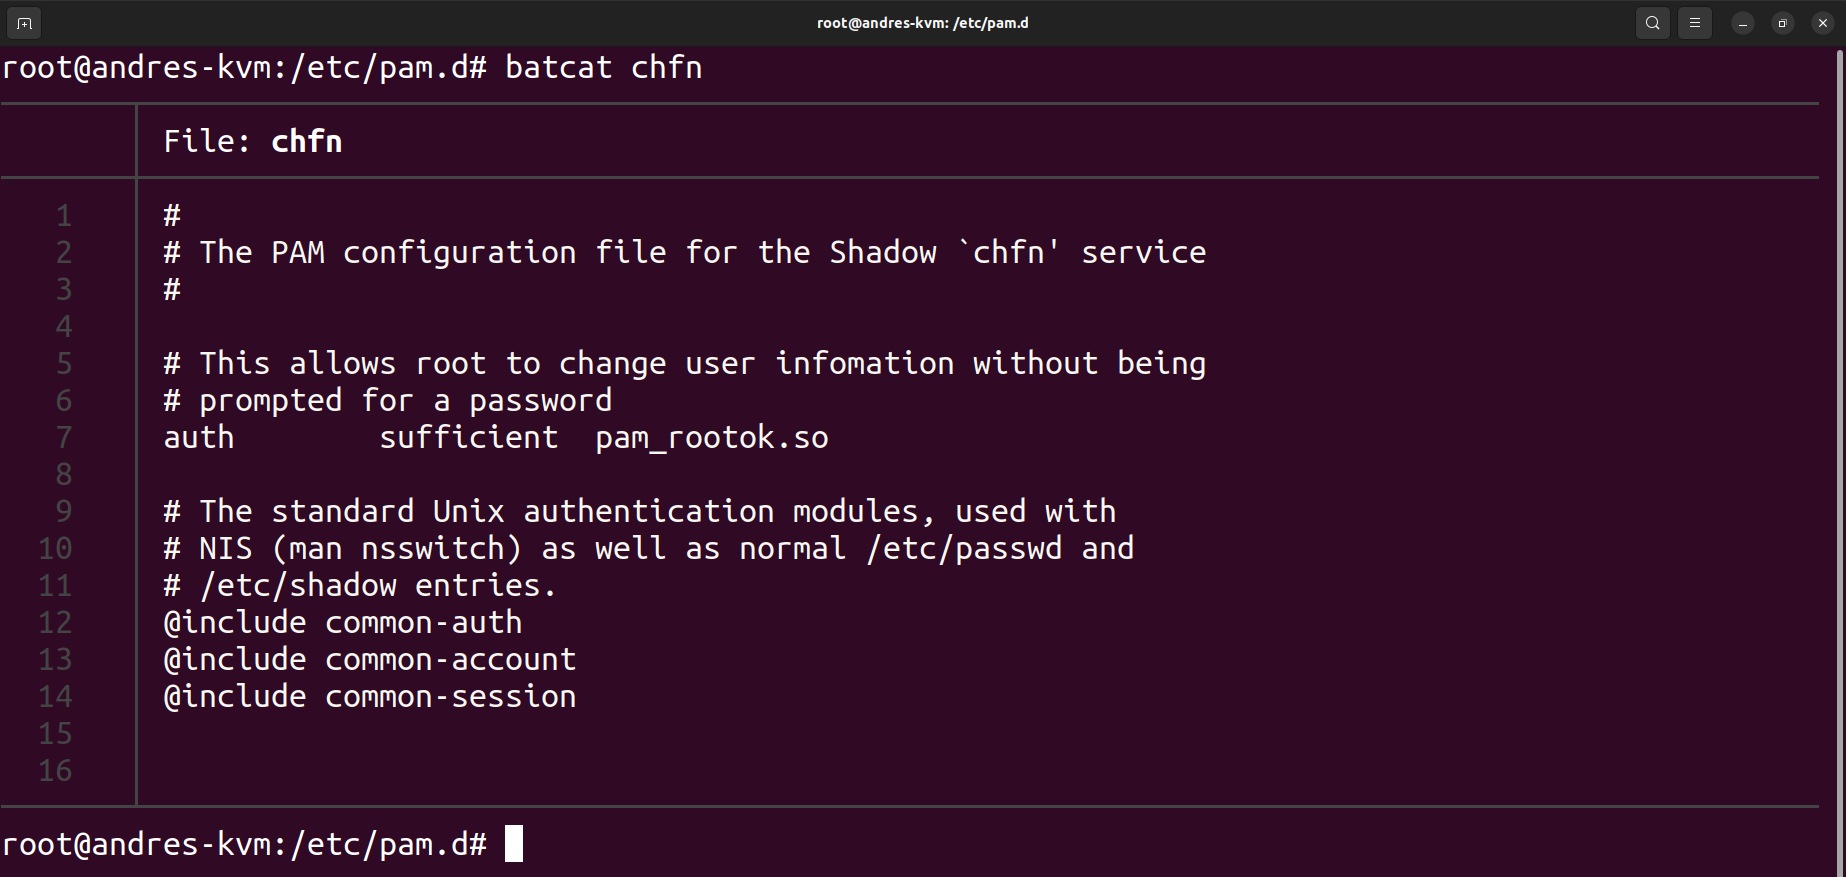
\includegraphics[width=\textwidth]{imagenes/pamchfn.png}
\end{figure}

La funcion de la linea 7 es para no pedir la contraseña al usuario root cuando esté usando este comando. Para ello, hace uso del campo de control sufficient, que hace que si tiene exito retorne sin ejecutar mas modulos. Ademas, hgace uso del modulo ``pam\_rootok.so'' que hace que solo tenga extio si el usuario tiene el UID a 0 (es el usuario root).

\subsection{/etc/pam.d/chsh}
El comando ``chsh'' permite cambiar la shell por defecto del usuario que lo invoca. Si no se le pasa ningun parametro se activa el modo interactivo para realizar el cambio de shell.

El contenido del archivo es el siguiente:

\begin{figure}[H]
    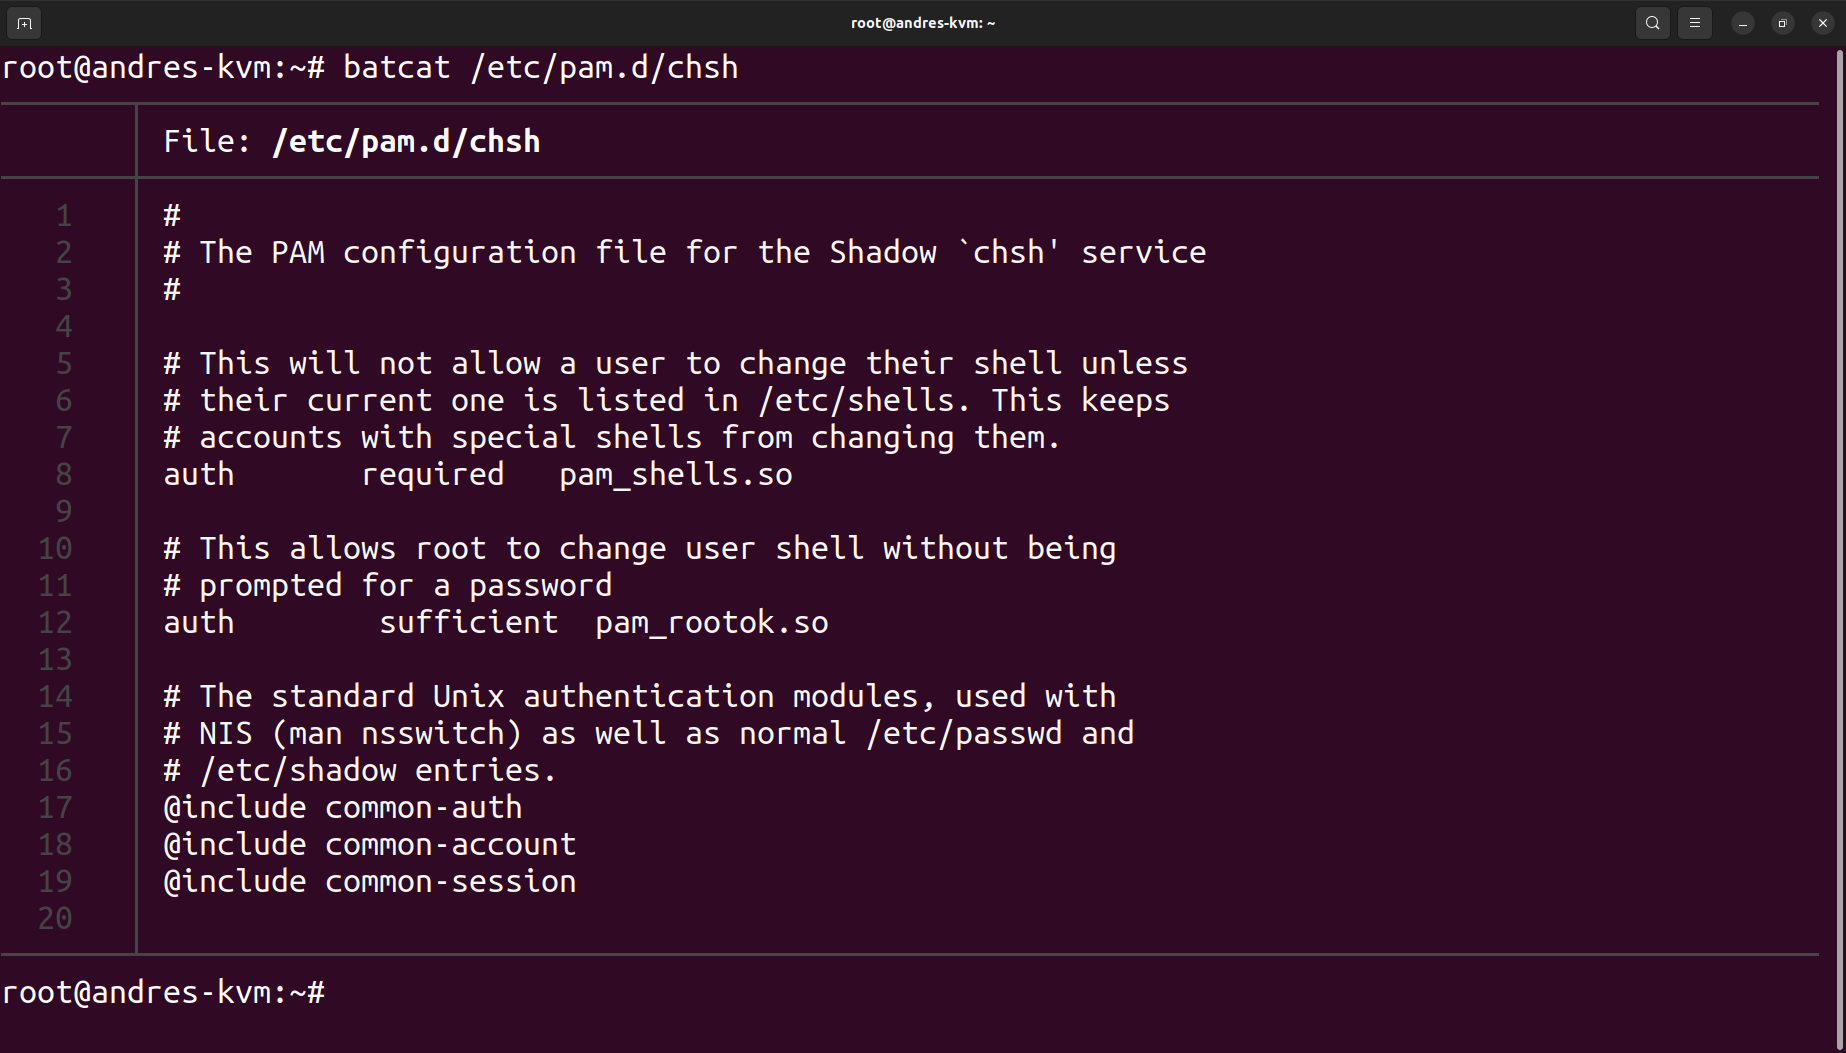
\includegraphics[width=\textwidth]{imagenes/pamchsh.png}
\end{figure}


Como se puede ver en la linea 8, esta llamada lo que hace es prohibir el cambio de shell a no ser que se encuentre listada en ``/etc/shells''. Esto se consigue mediante el campo de control ``required'', que provocará un fallo de autenticacion en el sistema (ejecutará la linea siguiente, pero al ser irrelevante, no pasa nada) si el modulo falla. Tambien se consguie mediente la llamada al modulo ``pam\_shells.so'', que hace que si la shell pasada como parametro no se encuentra en ``/etc/shells'' dé un fallo.

La funcion de la linea 12 es de permitir al superusuario cambiar la shell sin ser necesdario introducir la contraseña. Esto se realiza mediante el campo de control ``sufficient'' y el modulo ``pam\_rootok.so''. Con ``sufficient'', cuando la orden tiene exito retorna sin ejecutar los demas modulos \textbf{COMPROBAR AFIRMACION: (Como es el ultimo puede retornar sin prblema)}. Ademas, con el modulo ``pam\_rootok.so'' autoriza al usuario con el UID 0 (root).


\section{Quinto ejercicio}
\subsection{Apartado a}
Es necesario modificar el archivo PAM ``common-password'' y en Ubuntu 22.04 ya como primera linea aparece el uso del modulo ``pam\_pwquality''. 

Ahora bien si leemos el manual de este modulo con ``man 8 pam\_pwquality'' se puede ver que hay un argumento denominado ``minlen'' y que valor por defecto es 8. No obstante, no se puede bajar del valor 4, ya que es un limite que tiene ``Cracklib'' y mostrara que la contrasñae es muy corta. Por eso, voy a poner el limite a \textbf{15 caracteres}.

\begin{figure}[H]
    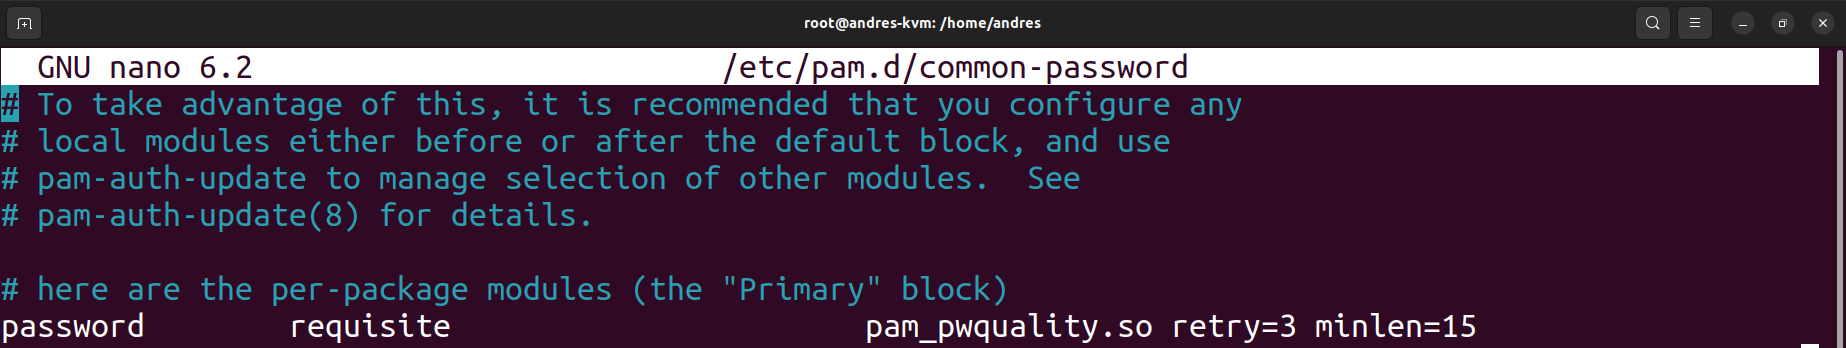
\includegraphics[width=\textwidth]{imagenes/passwordminlen15.png}
\end{figure}

Y ahora al usar el comando ``passwd'' y poner una contraseña con menos de 15 palabras, muestra un error:

\begin{figure}[H]
    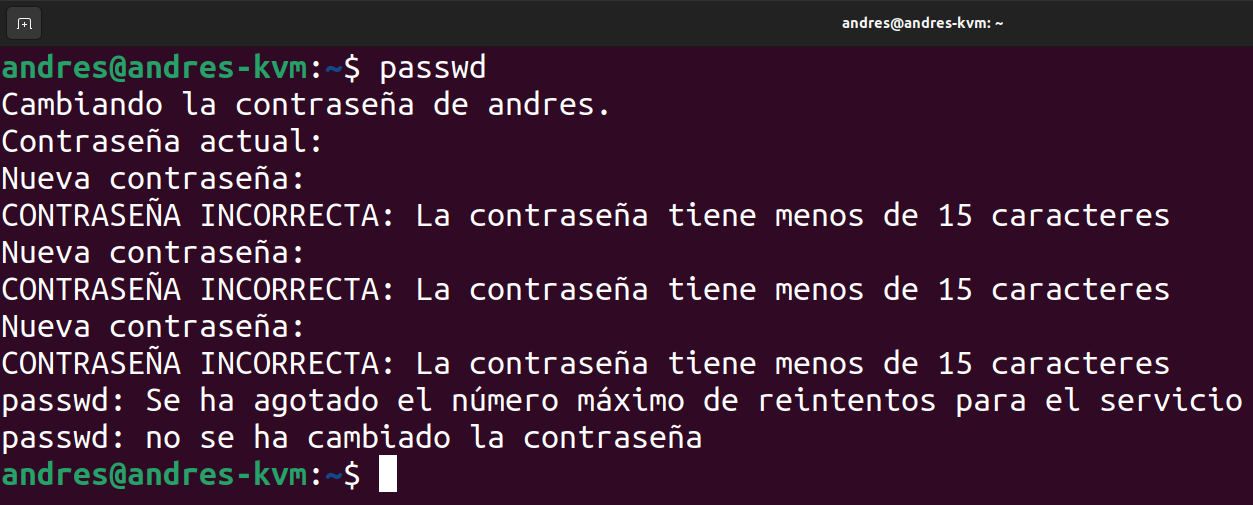
\includegraphics[width=\textwidth]{imagenes/passwordminlen15passwd.png}
\end{figure}

Y al agotarse los intentos (que son 3) se sale del programa.
\subsection{Apartado b}
En esta parte he restringido el acceso al comando ``su'' para así evitar que un usuario que ponga el comando sin ``sudo'' pueda entrar. Si ponen ``sudo su'' sí van a poder entrar, pero esto es así ya que son usuarios administradores (y es una decisión de diseño, ya que en otro caso no podría usar nadie ``sudo''), en ese caso lo recomendable es deshabilitar el acceso al grupo ``sudo'' (en el caso de Ubuntu) para que no lo pueda usar (editando el archivo sudoers mediante el comando ``visudo'').

Para conseguir esto, es neceasrio modificar el arcvhio ``/etc/pam.d/su'' y añadir la siguiente línea al principio:

\begin{figure}[H]
    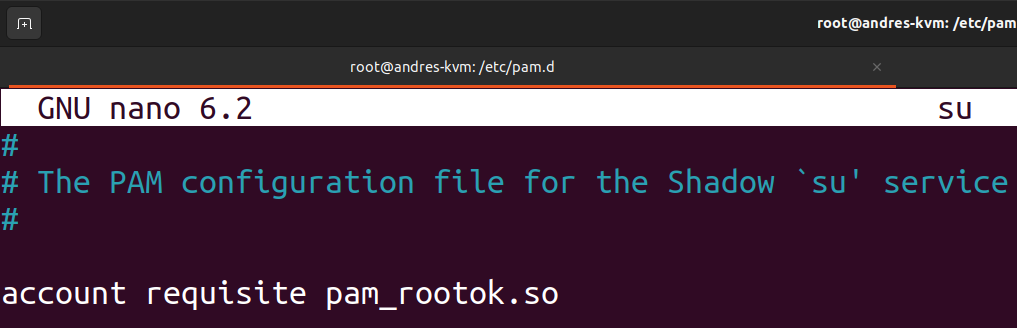
\includegraphics[width=\textwidth]{imagenes/sudeny.png}
\end{figure}

Ahora, al ejecutar el comando ``su'' con un usuario nomral aparece lo siguiente:

\begin{figure}[H]
    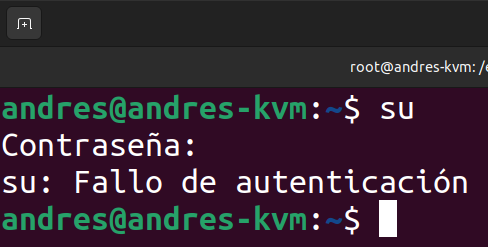
\includegraphics[width=\textwidth]{imagenes/sudenyuser.png}
\end{figure}


En cambio, si el usuario puede usar ``sudo'', si puede acceder.

\begin{figure}[H]
    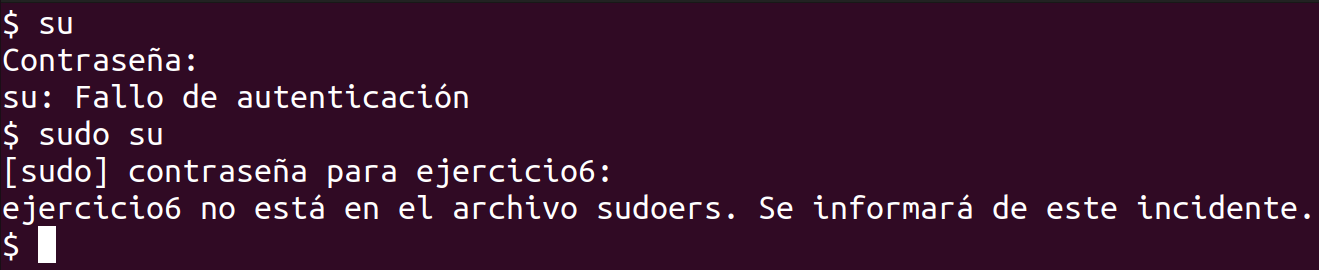
\includegraphics[width=\textwidth]{imagenes/sudenyuserprueba.png}
    \caption{el usuario que se ha creado en esta practica no tiene permisos de sudo y por tanto no puede entrar de ninguna manera}
\end{figure}

La línea que he añadido lo que hace es comproba que la cuenta sea root (UID=0) y en caso de no serlo, no sigue ejecutando el archivo provocando un error de autenticación.


\section{Sexto ejercicio}
En Ubuntu 22.04 los cambios de contraseña no se almacenan en ``/var/log/messages'', sino en ``/var/log/auth.log''. \href{https://ubuntu.com/tutorials/viewing-and-monitoring-log-files#2-log-files-locations}{Enlace} a la guía.


Voy a crear el usuario ``ejercicio6'' y le voy a cambiar la contraseña:

\begin{figure}[H]
    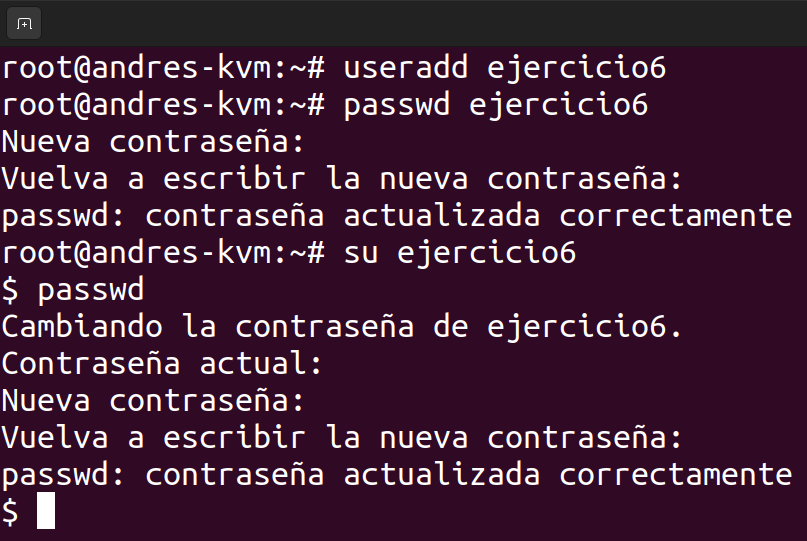
\includegraphics[width=\textwidth]{imagenes/createejercicio6.png}
\end{figure}

Y ahora, al mostrar el archivo ``/var/log/auth.log'' aparecen las siguientes lineas:

\begin{figure}[H]
    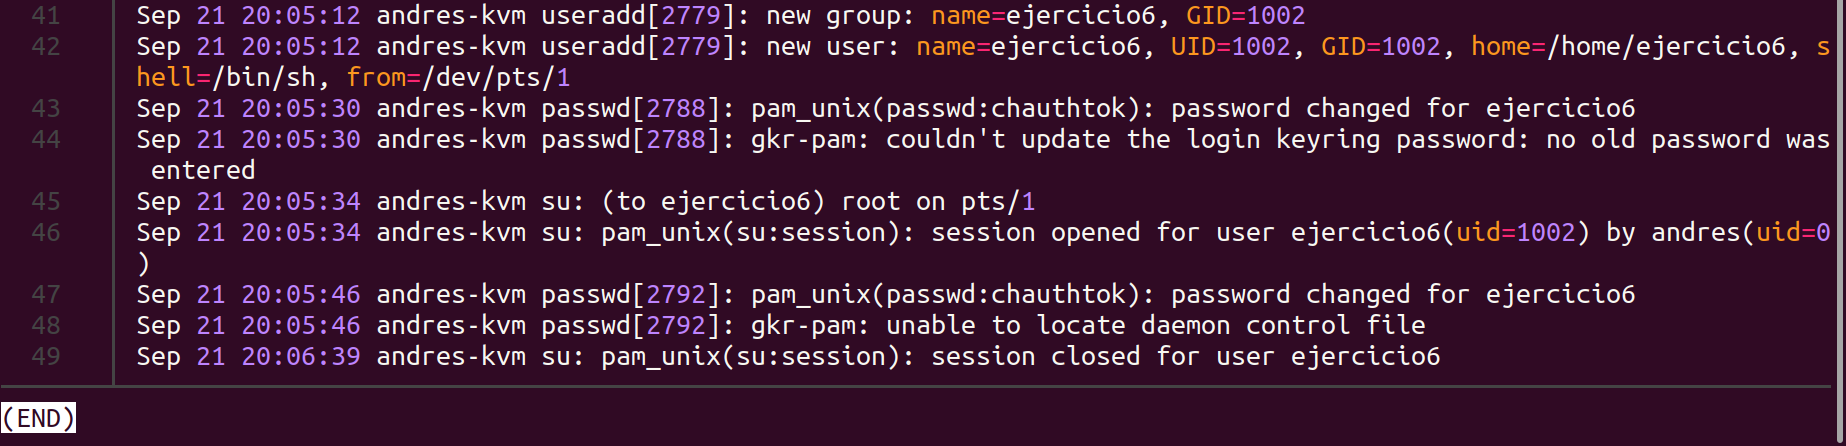
\includegraphics[width=\textwidth]{imagenes/authcreateejercicio6.png}
\end{figure}

\section{Séptimo ejercicio}
Para empezar, el propio archivon de sudoers recomienda usar la orden ``visudo''. POr tanto, es necesario usar ``visudo'' para que no haya problemas después. Además, por defecto usa el editor ``vi'', esto se puede cambiar usando el comando siguiente:

\verb|EDITOR=nano visudo|

Ahora, voy a asignarle permisos para usar sudo al usuario ``prueba'' que no se encuentra en el grupo ``sudo'', que es el que usa Ubuntu para dar permisos.

\begin{figure}[H]
    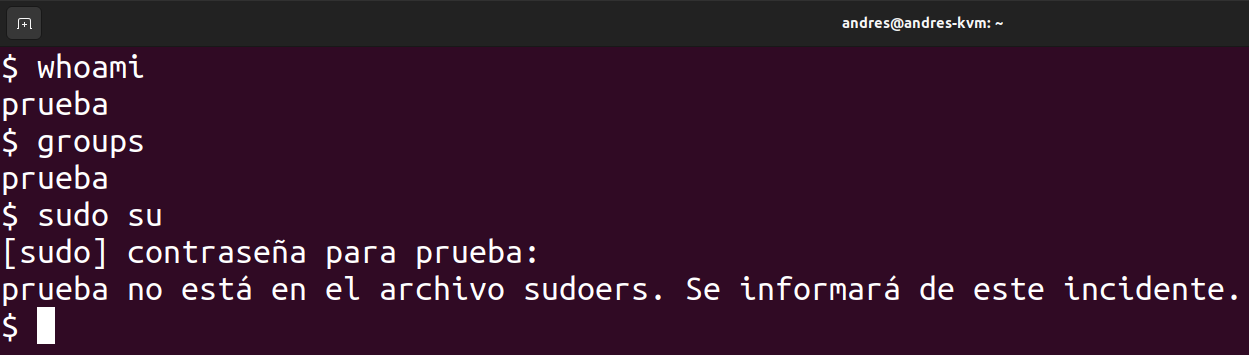
\includegraphics[width=\textwidth]{imagenes/sudoprueba.png}
\end{figure}

Si añadimos la siguiente linea en el archivo ``sudoers'' tendremos acceso con sudo:

\begin{figure}[H]
    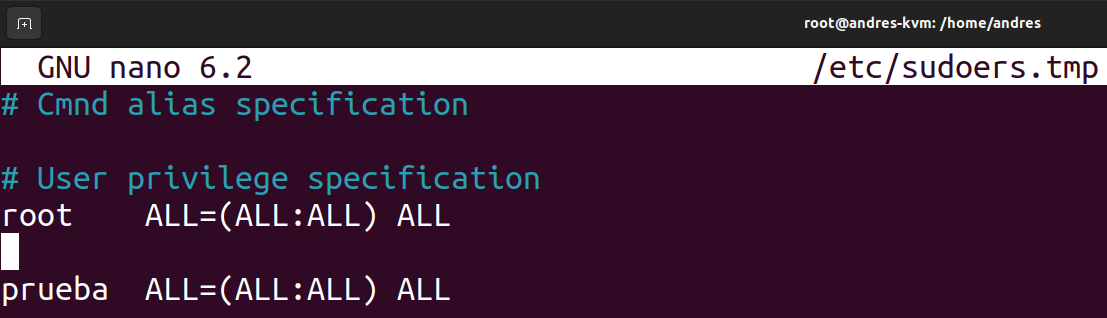
\includegraphics[width=\textwidth]{imagenes/sudoersprueba.png}
\end{figure}


Y ahora al hacer una prueba se puede ver que ya funciona:

\begin{figure}[H]
    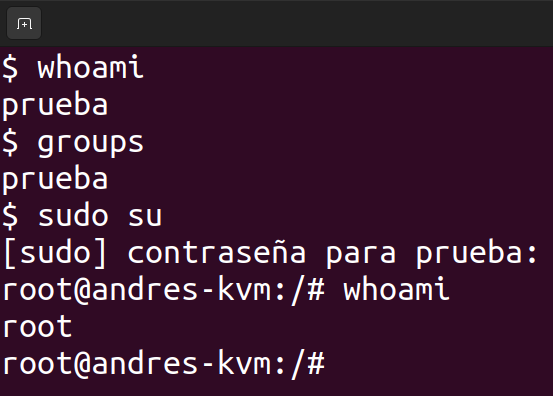
\includegraphics[width=\textwidth]{imagenes/sudopruebaok.png}
\end{figure}

\section{Octavo ejercicio}
Voy a examinar cada uno de los archivos y comprobar que se registran eventos que realizaré. Para ello, voy a dividir la explicacion en subsecciones para cada uno de los archivos.

\subsection{/var/log/lastlog}
ESte archivo almacena informacion sobre le ultimo inicio de sesion de los usuarios. Para acceder a la informacion es necesairio utilizar el comando ``lastlog'':

\begin{figure}[H]
    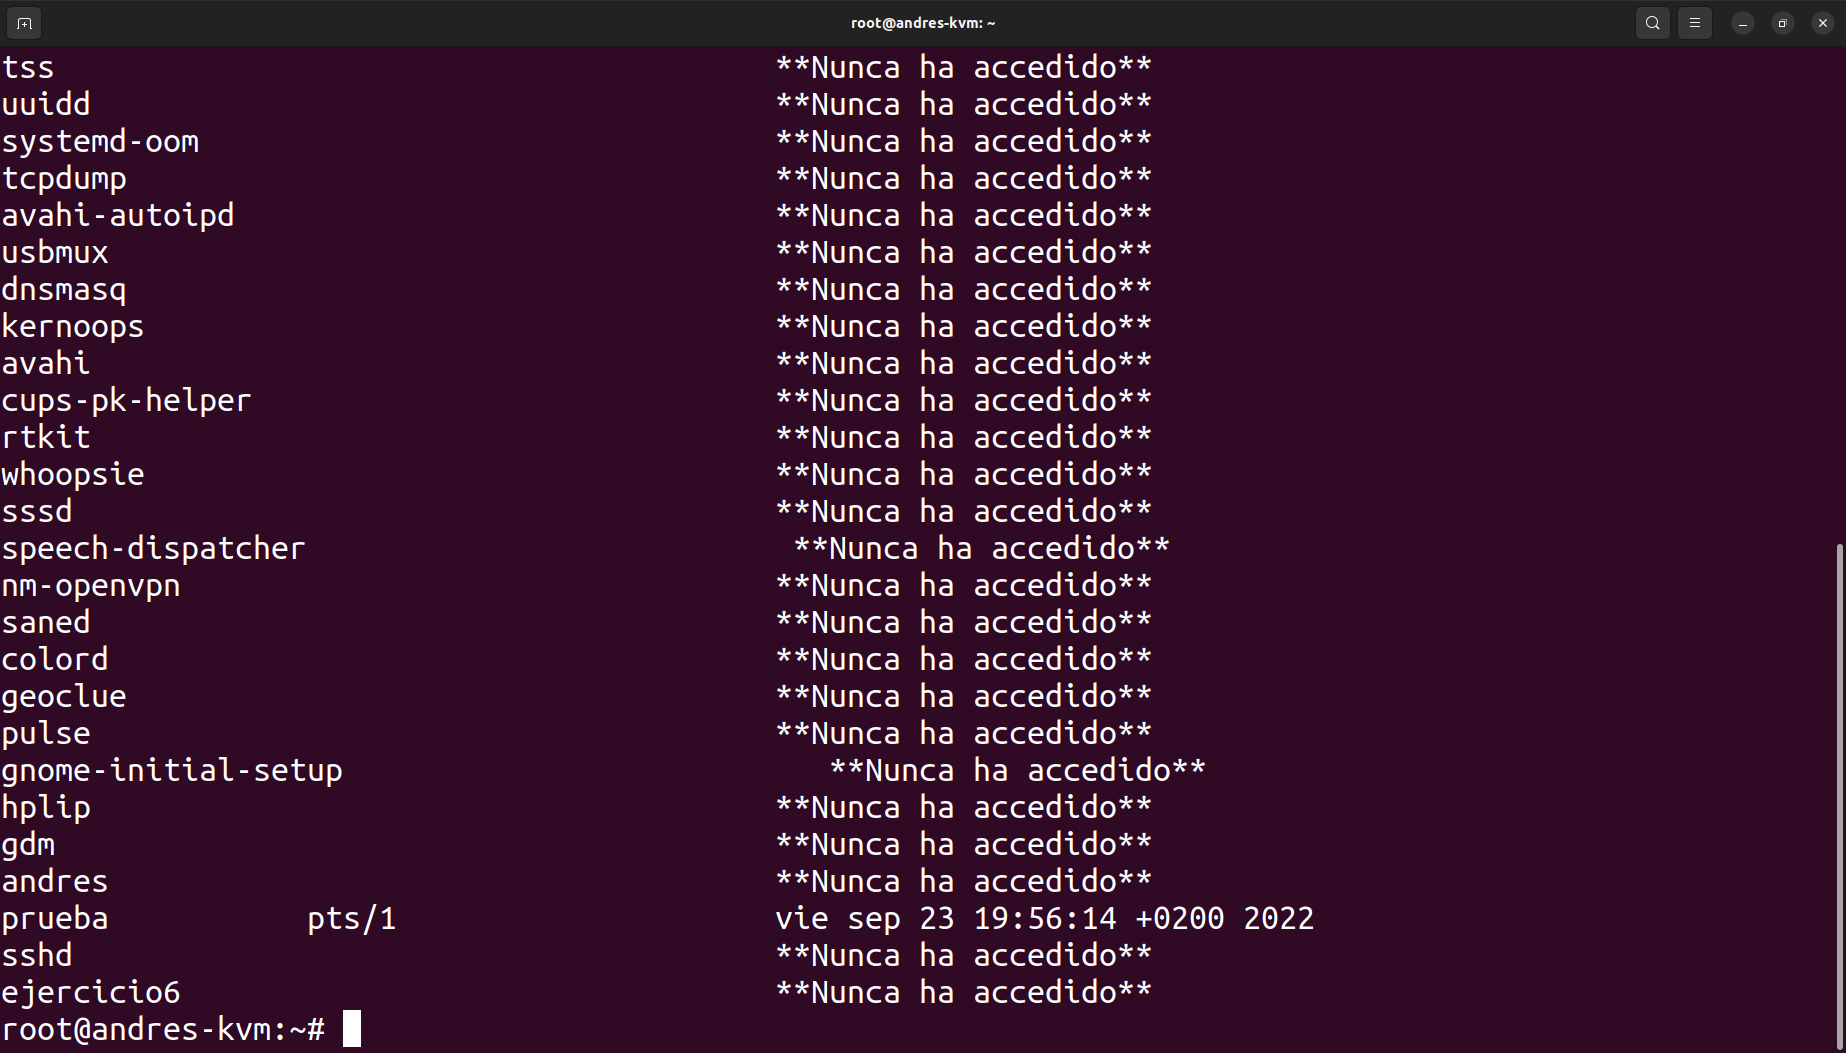
\includegraphics[width=\textwidth]{imagenes/lastlogejercicio6never.png}
\end{figure}

Como se puede ver, el usuario ``ejercicio6'' nunca ha iniciado sesion en el sistema. Ahora si inicio sesion y vuelvo a usar la orden ``lastlog'' aparece lo siguiente:

\begin{figure}[H]
    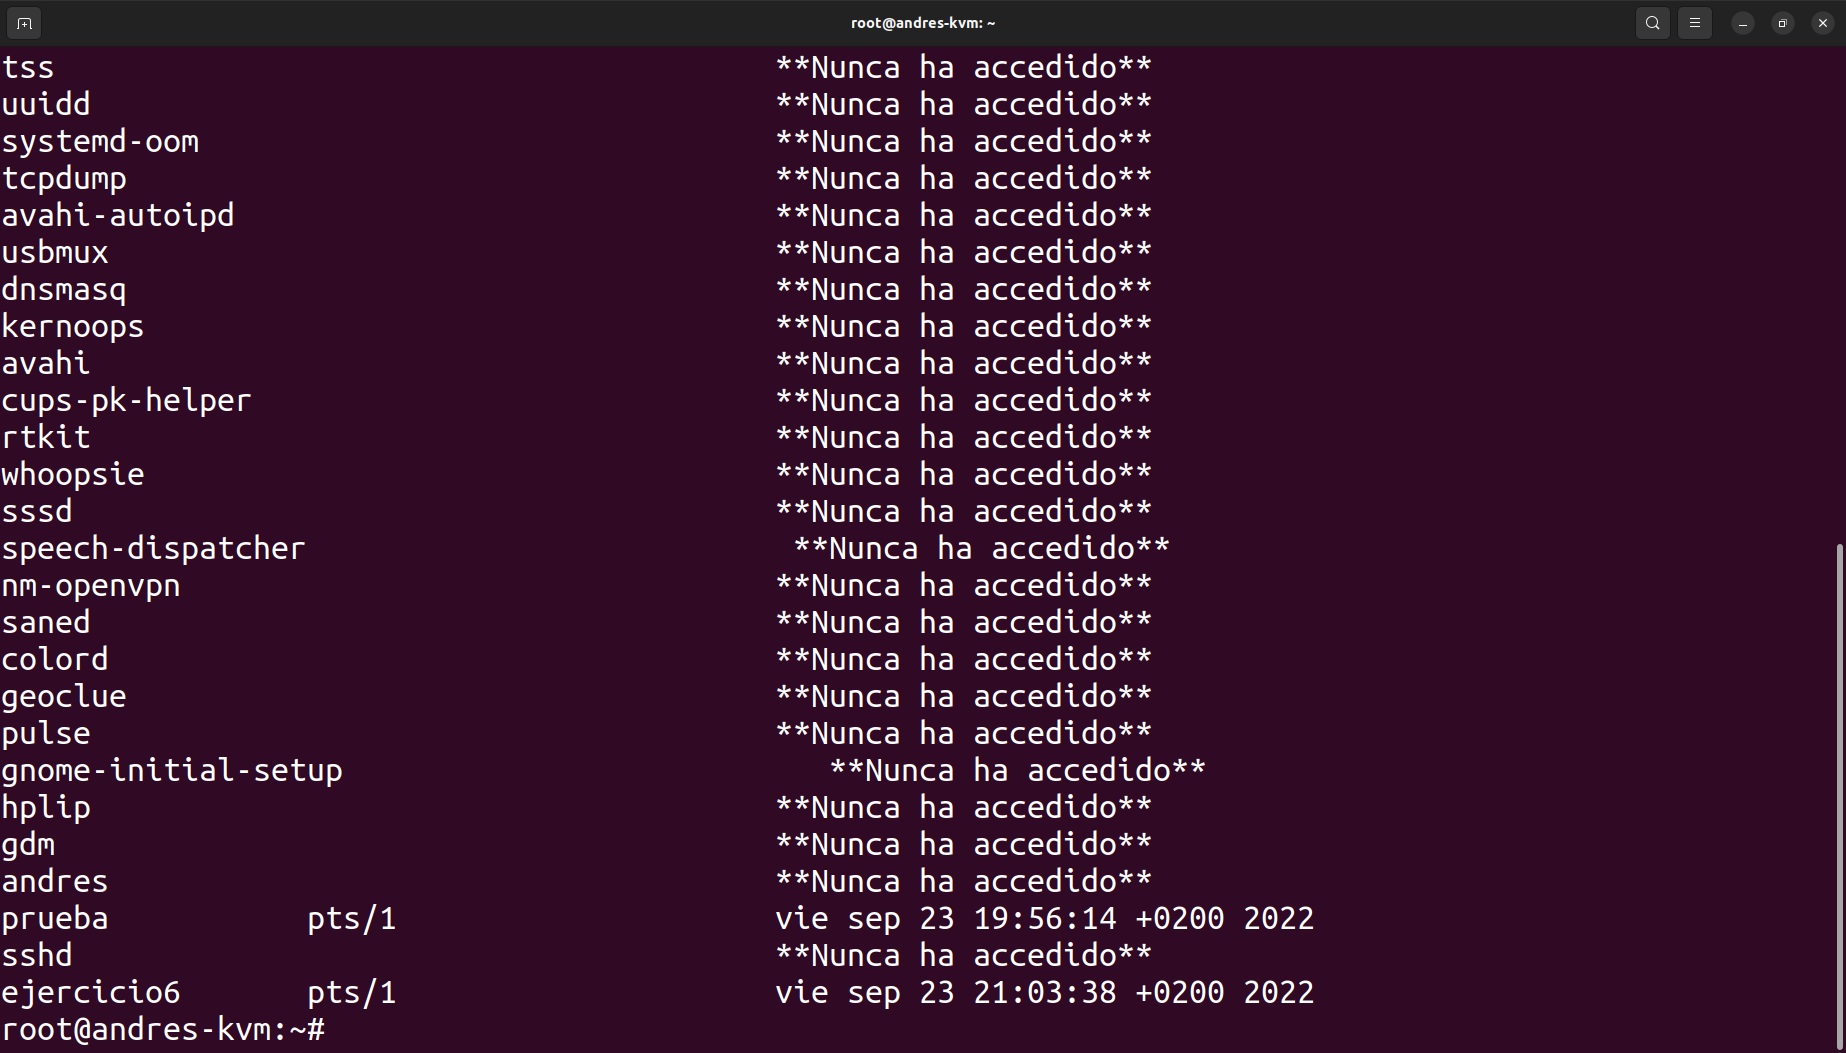
\includegraphics[width=\textwidth]{imagenes/lastlogejercicio6ok.png}
\end{figure}

Ahora como se puede ver aparece la fecha del ultimo inicio de sesion del usuario ``ejercicio6''.

\subsection{/var/log/wtmp}
Almacena los login y logout de los distintos usuarios del sistema. Se accede con el comando ``last''. 

\begin{figure}[H]
    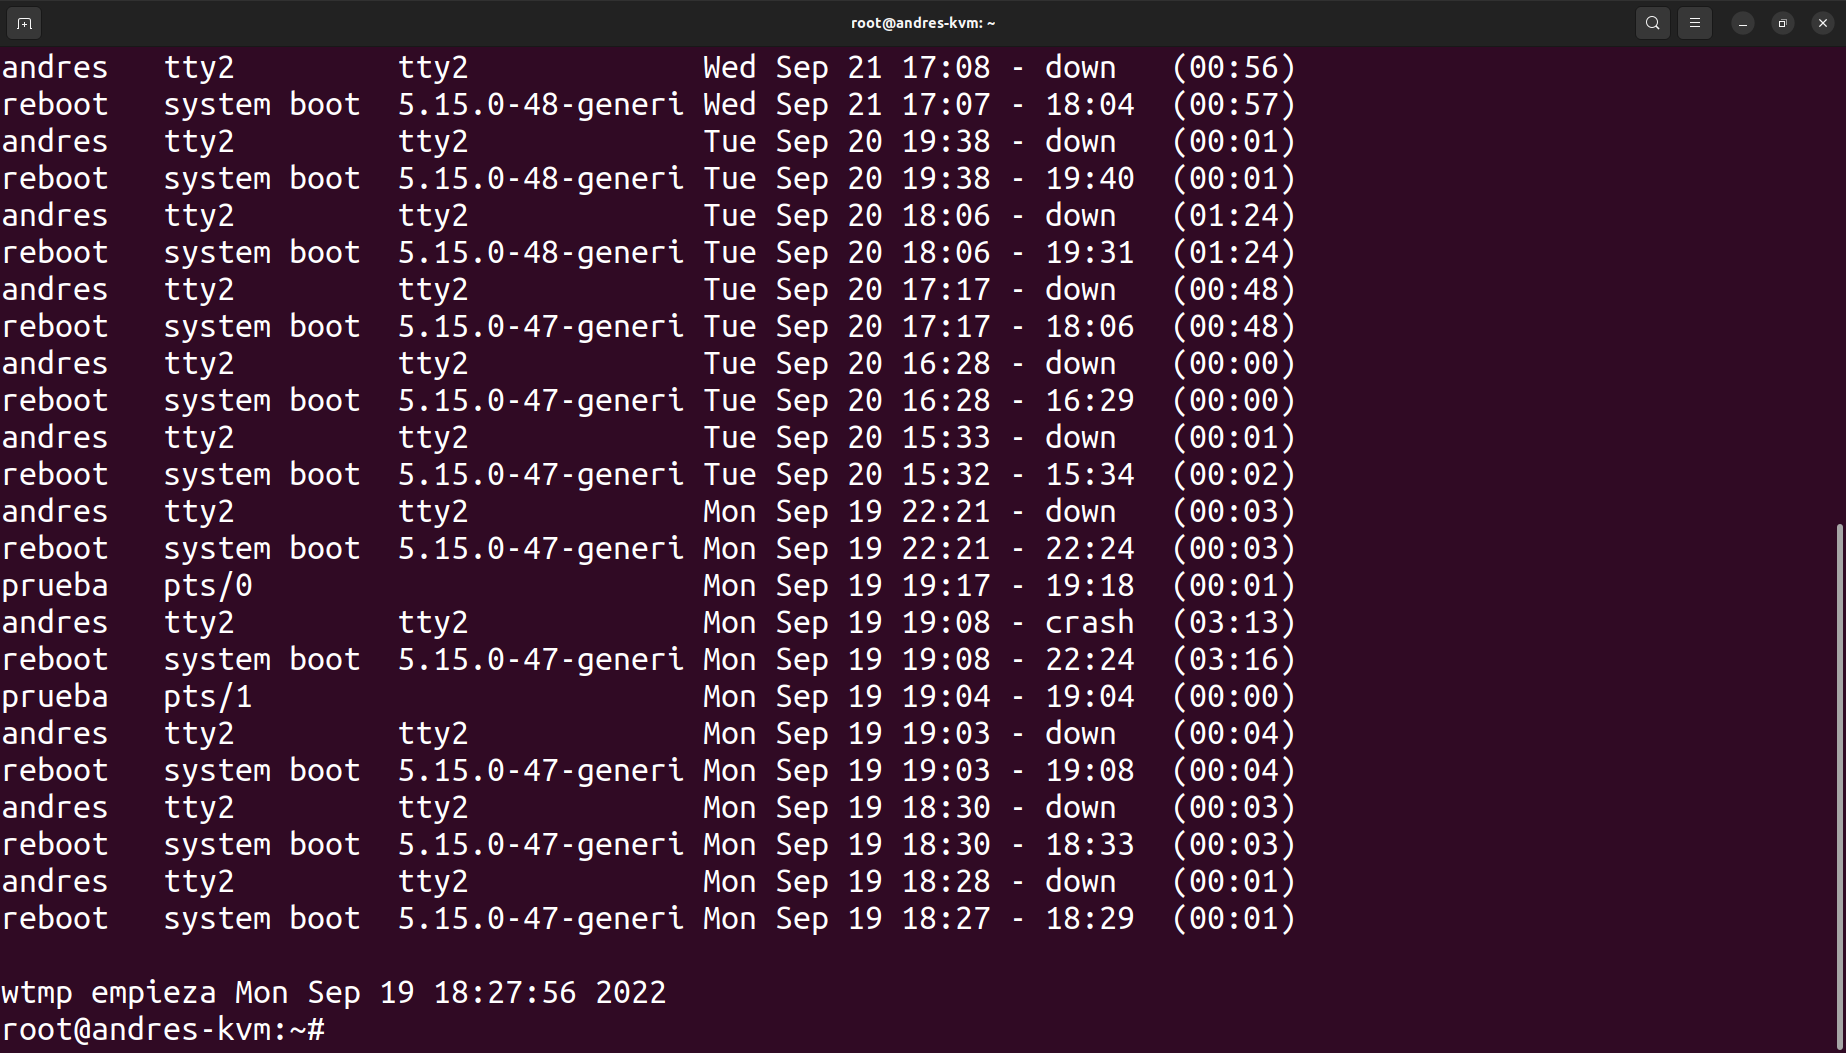
\includegraphics[width=\textwidth]{imagenes/lastnormal.png}
\end{figure}

Ahora con el comando ``last --since today'' muestra solo la informacion de hoy.

\begin{figure}[H]
    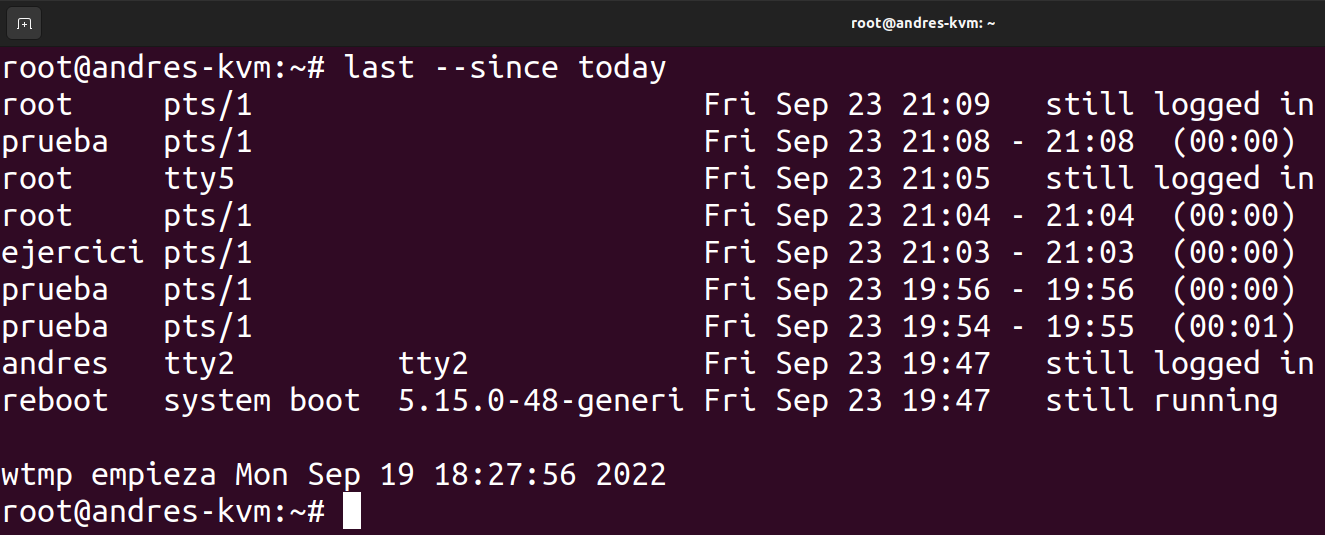
\includegraphics[width=\textwidth]{imagenes/lasttoday.png}
\end{figure}

Y ahora voy a inicar sesion con el usuario ``prueba'' y lohout para ver como se almacena la informacion:

\begin{figure}[H]
    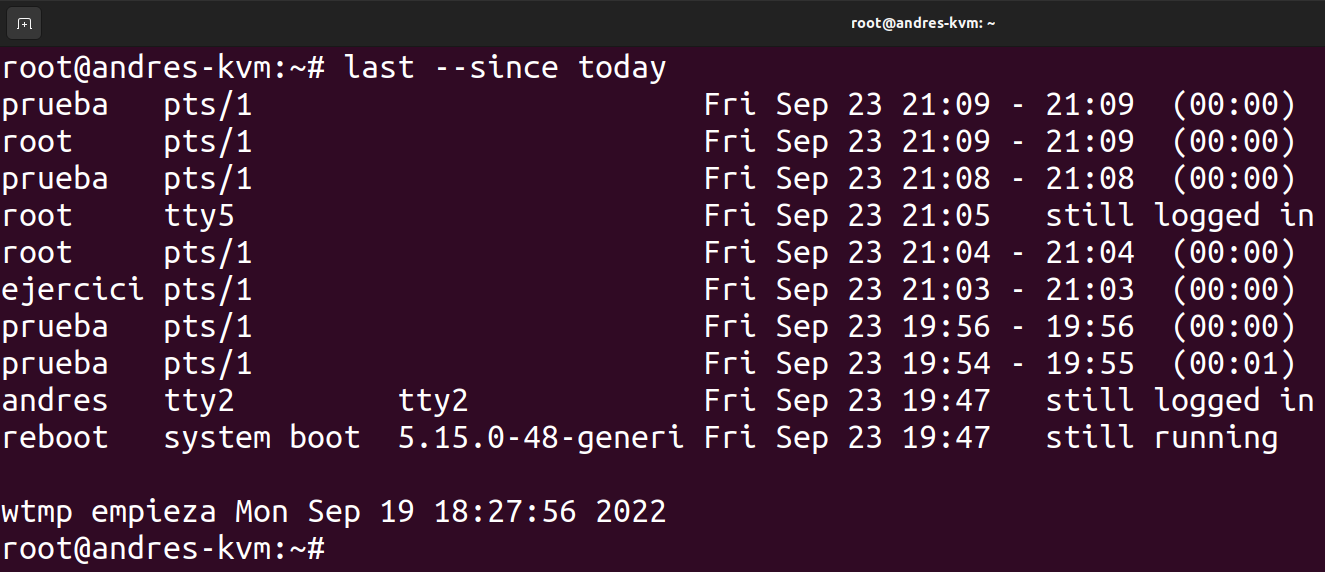
\includegraphics[width=\textwidth]{imagenes/lasttodayprueba.png}
\end{figure}

\subsection{/var/log/utmp}
Muestra los usuarios que estan \textit{loggeados} en el sistema. Se puede obtener esta cinfromacion con la orden ``who''.

\begin{figure}[H]
    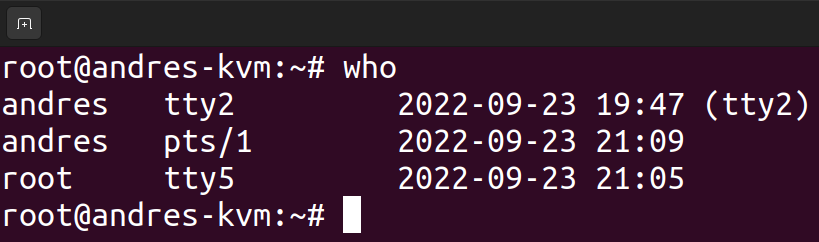
\includegraphics[width=\textwidth]{imagenes/whonormal.png}
\end{figure}

AHora si inicio sesion con el usuario ``prueba'' deberia aparecer con el comando anterior:

\begin{figure}[H]
    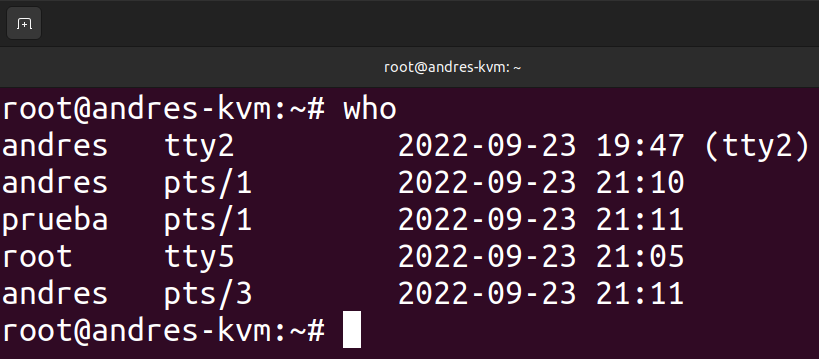
\includegraphics[width=\textwidth]{imagenes/whoprueba.png}
\end{figure}

\subsection{/var/log/btmp}
Muestra los intentos fallidos de inicio de sesion en el sismtea. Se puede obtener con la orden ``lastb''.

\begin{figure}[H]
    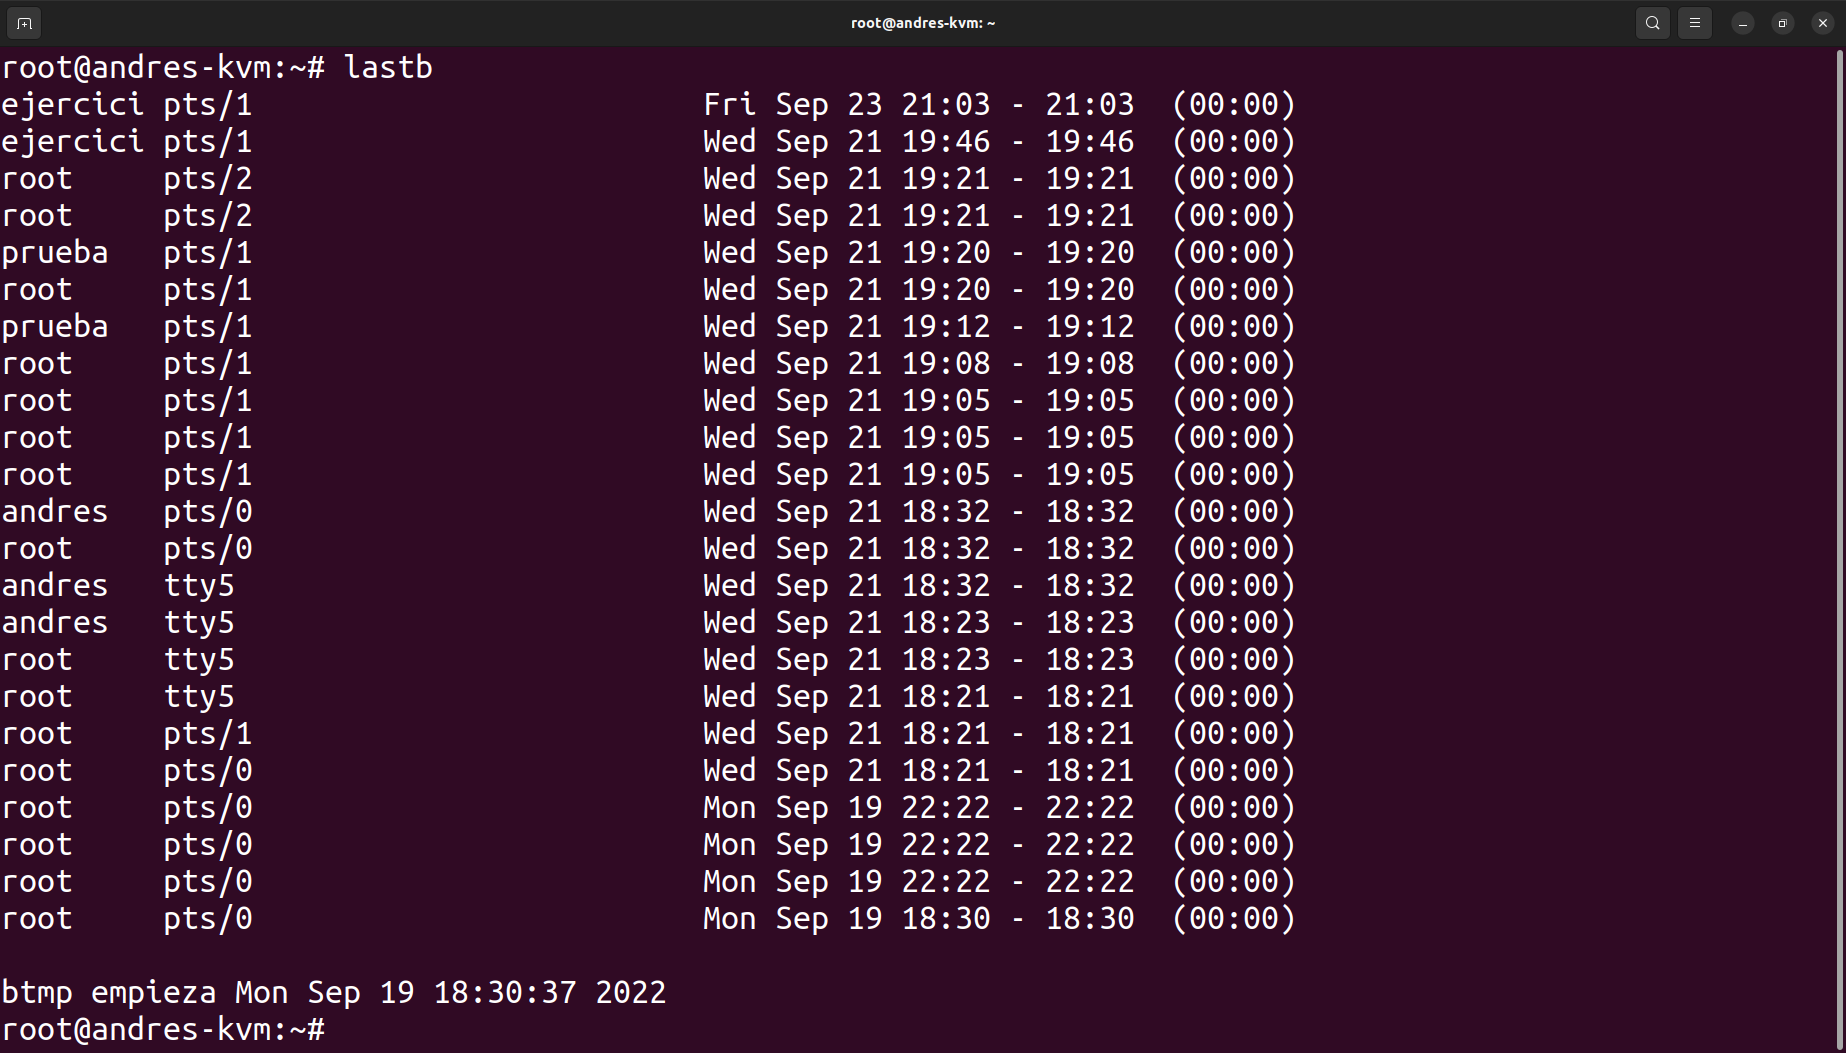
\includegraphics[width=\textwidth]{imagenes/lastbnormal.png}
\end{figure}

Ahora, si hago que fallo el inicio de sesion del usuario ``prueba'' deberia de salir:

\begin{figure}[H]
    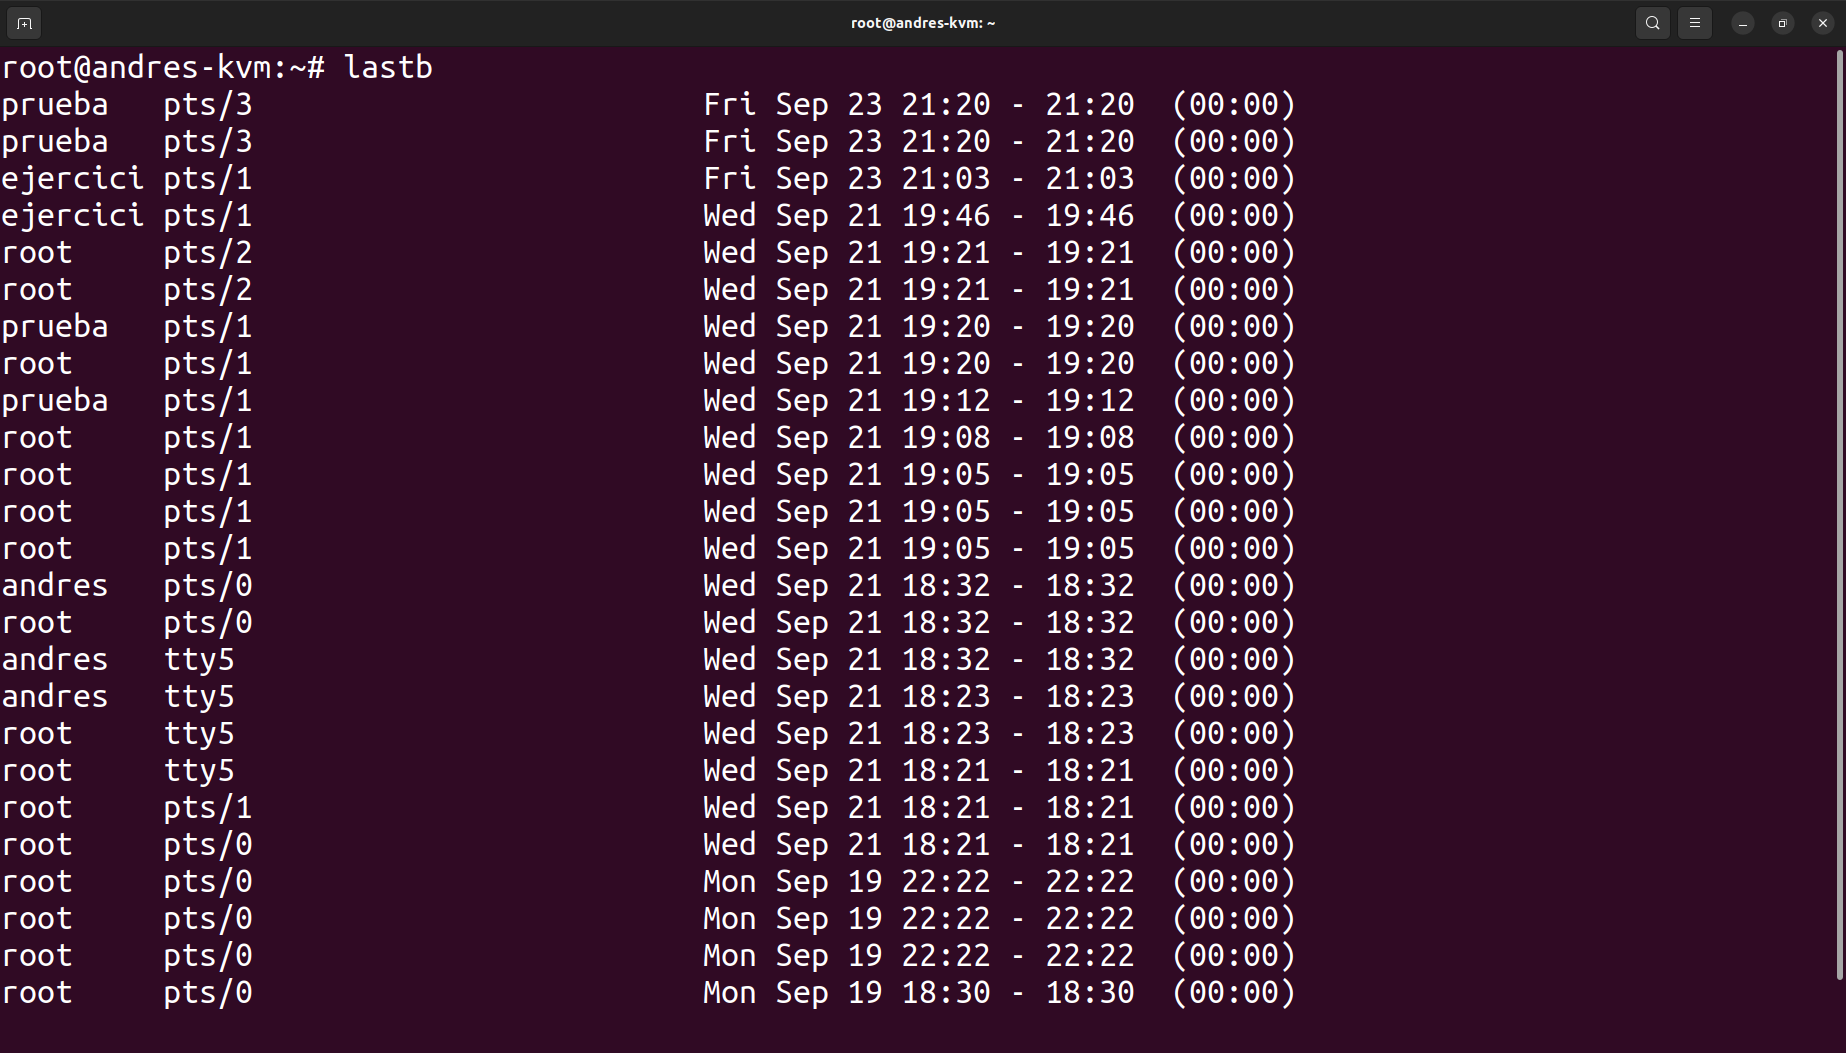
\includegraphics[width=\textwidth]{imagenes/lastbpruebafirst.png}
    \caption{Se puede ver que las dos primeras lineas pertenecen a intentos de login con le usuario ``prueba''.}
\end{figure}

\subsection{/var/log/sudo}
Este archivo, al menos en Ubuntu, no existe, por tanto no puedo mostrar informacion al respecto sobre la actividad del uso de ``sudo''.
\subsection{/var/log/messages}
En Ubuntu (no sé si en otras distribuciones también) ya no existe este archivo porque duplicaba informacion con ``/var/log/syslog''. Por tanto, voy a mostrar este archivo:

\begin{figure}[H]
    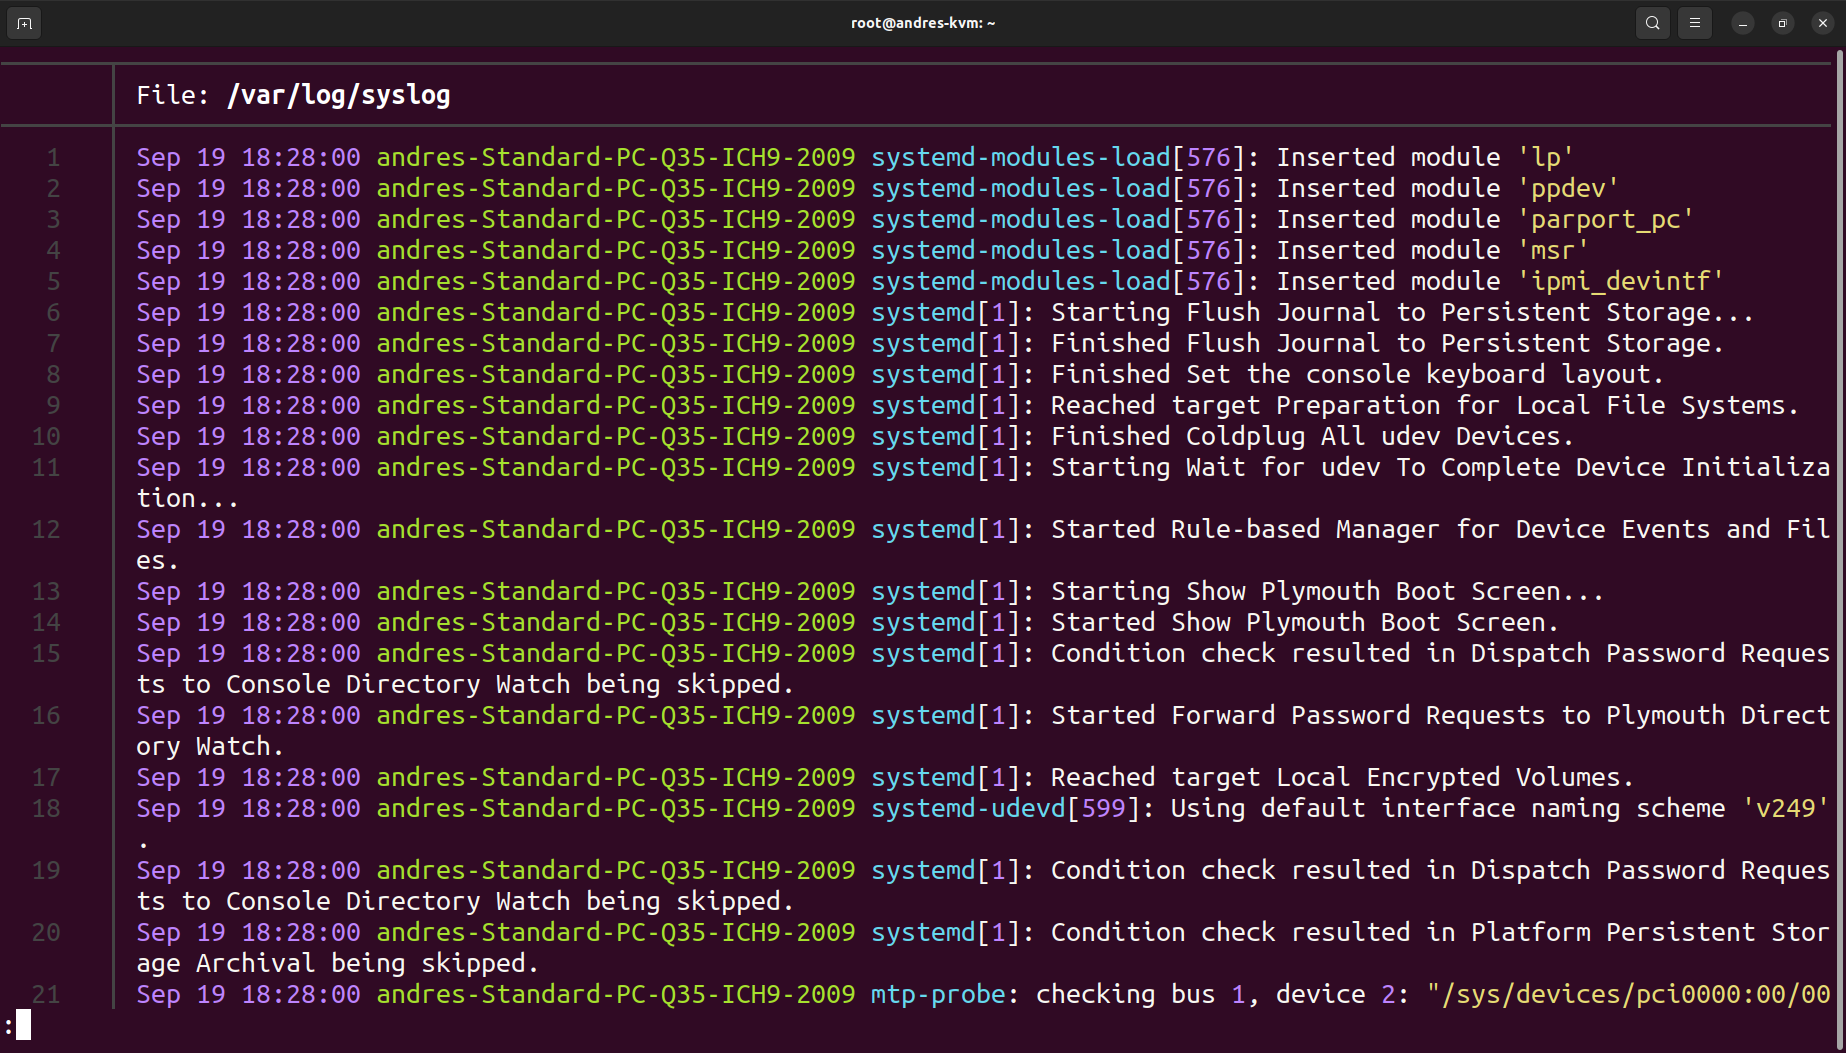
\includegraphics[width=\textwidth]{imagenes/syslog.png}
\end{figure}

\subsection{Noveno ejercicio}
\subsection{PC de mi casa}
Para comprobar los intentos de inicio de sesion fallidos en el ordenador de mi casa, voy a usar ``lastb'':

\begin{figure}[H]
    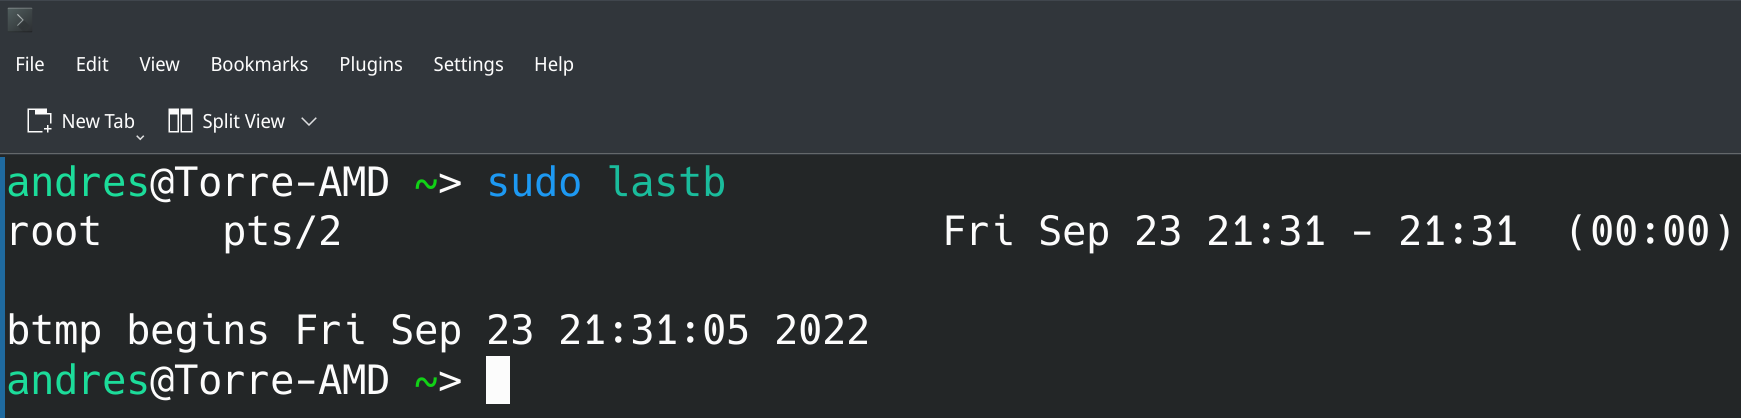
\includegraphics[width=\textwidth]{imagenes/lastbcasa.png}
\end{figure}

Como se puede observar, el unico intento fallido de inicio de sesion que he tenido ha sido provocado por mi en el momento de hacer esta parte del ejercicio.

Ahora, muestro con el comando ``last'' los login y logout del sitema:

\begin{figure}[H]
    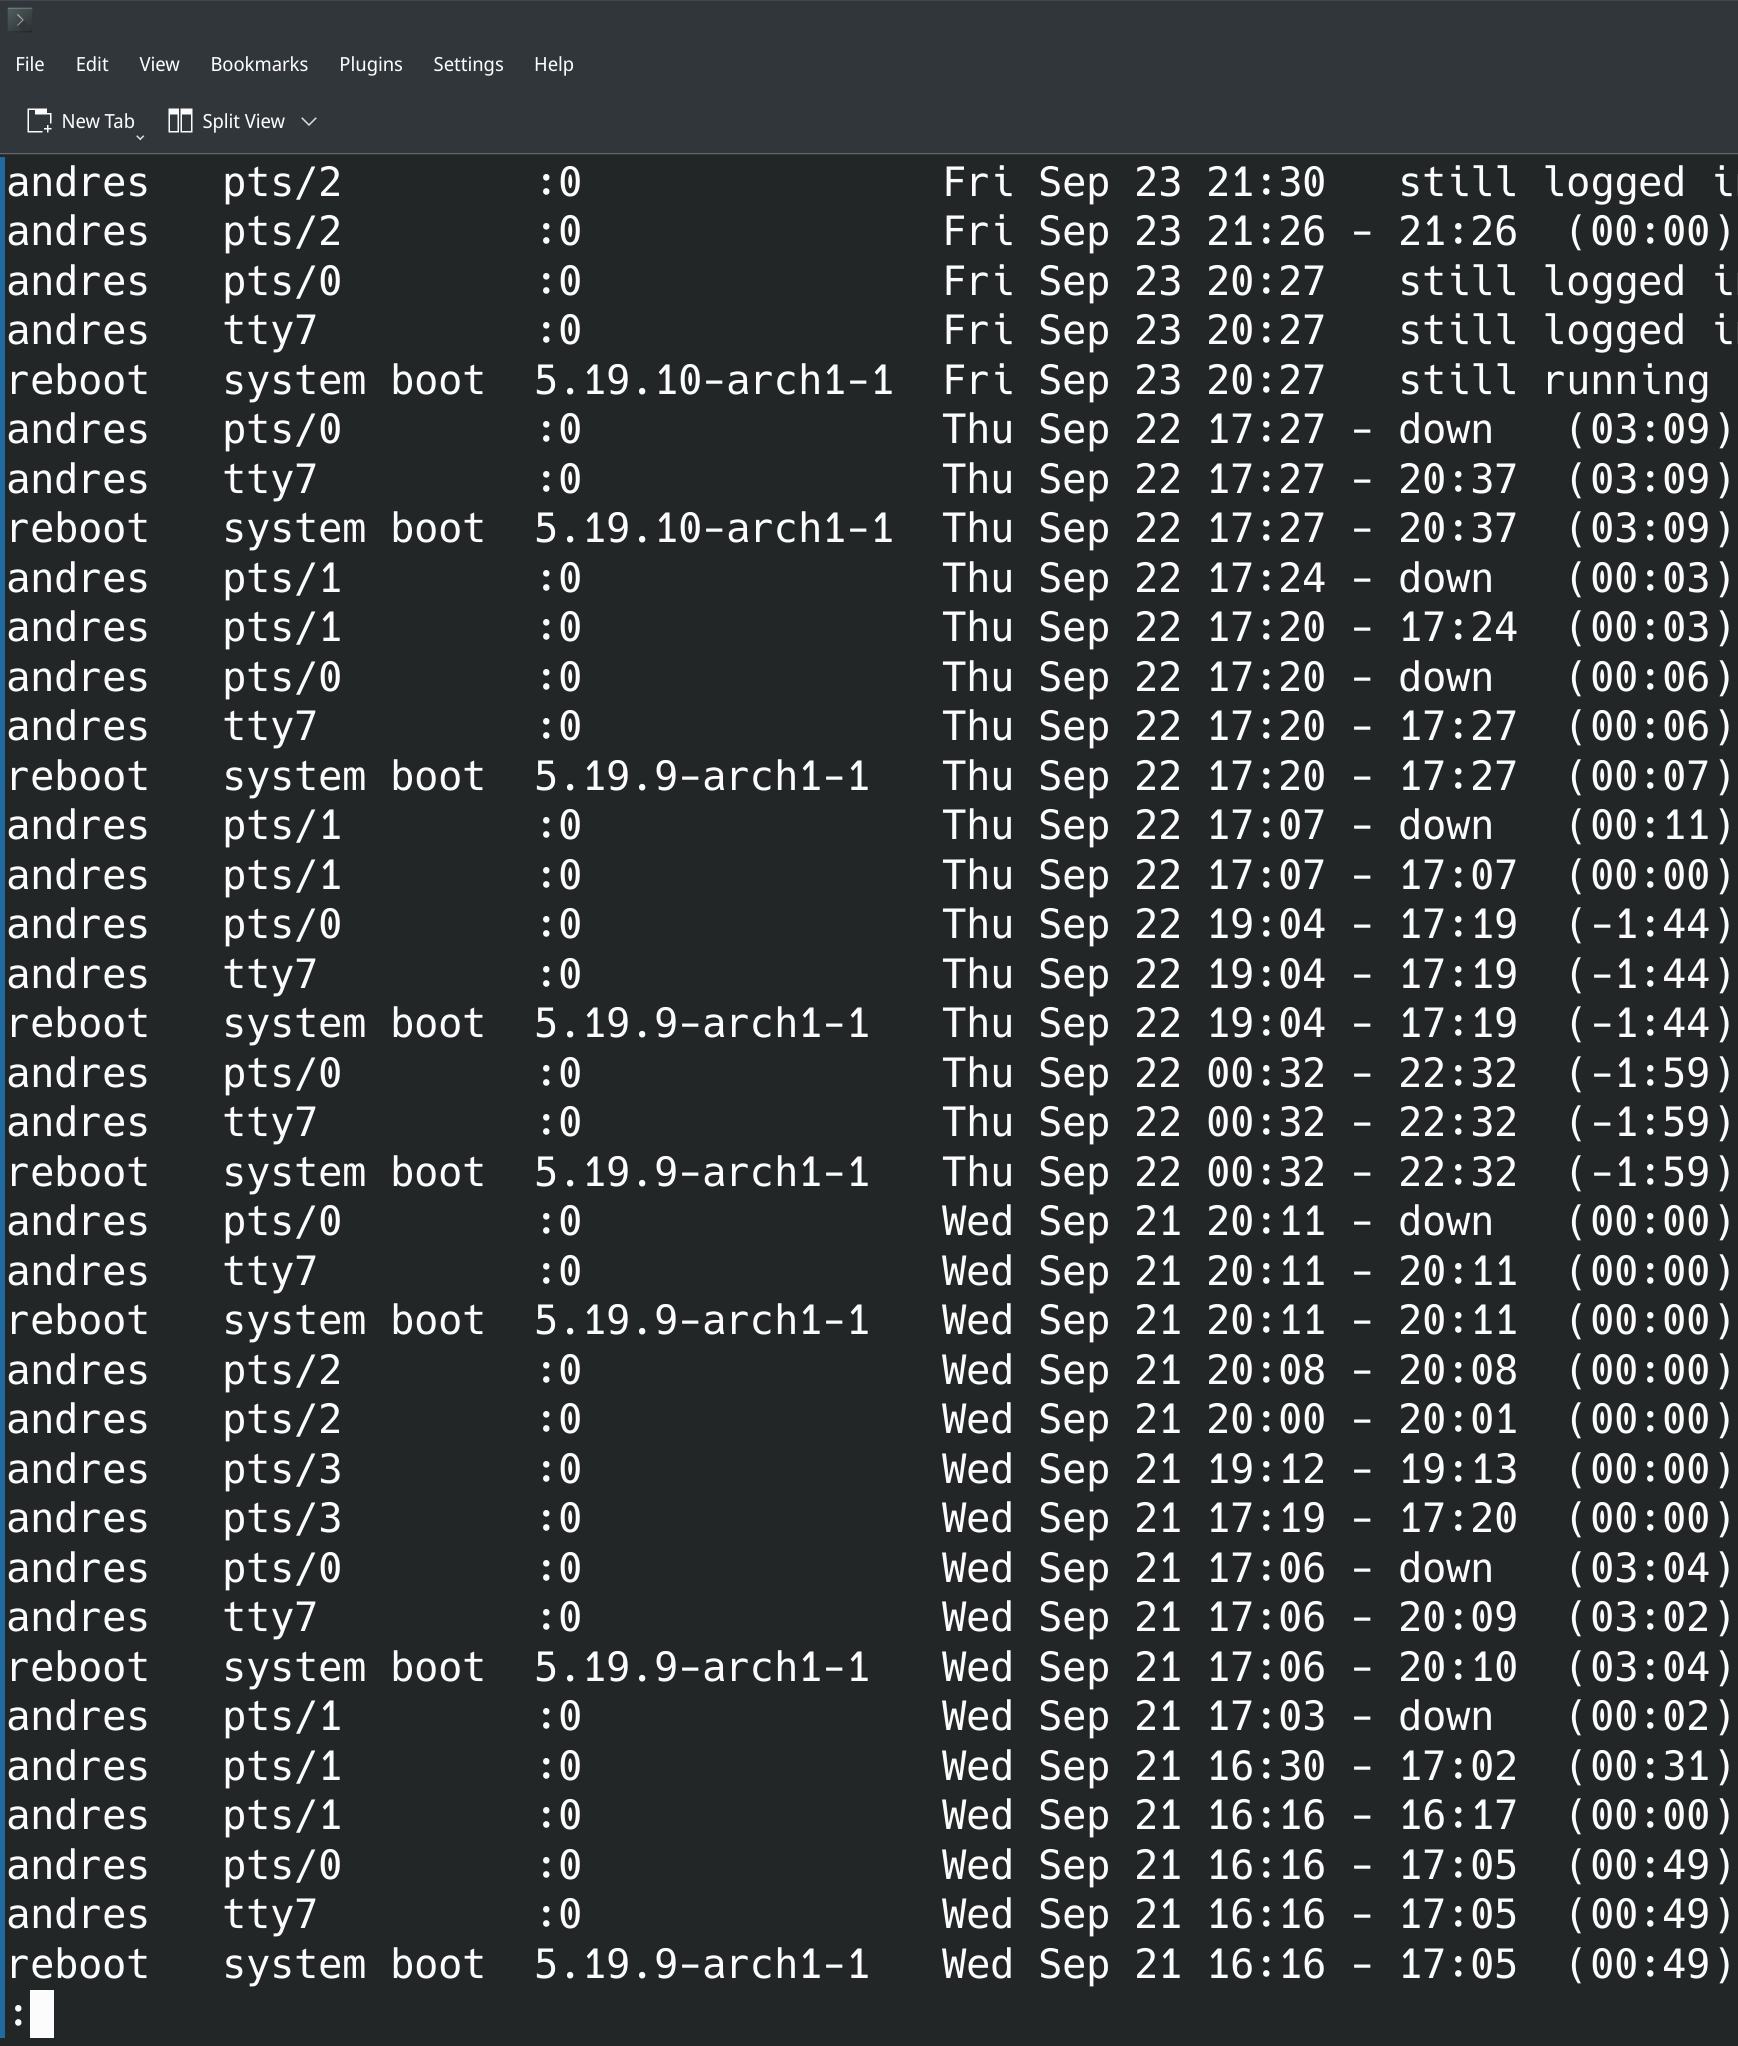
\includegraphics[width=\textwidth]{imagenes/lastcasa.png}
\end{figure}

POr lo que puedo ber, no ha habido ningun inicio en el ssistema por ssh (se mostraria en la tercera columna la direccion IP del que lo ha intentado).

POr ultimo, con la orden ``lastlog'' muestro los inicios de sesion producidos en el sistema.

\begin{figure}[H]
    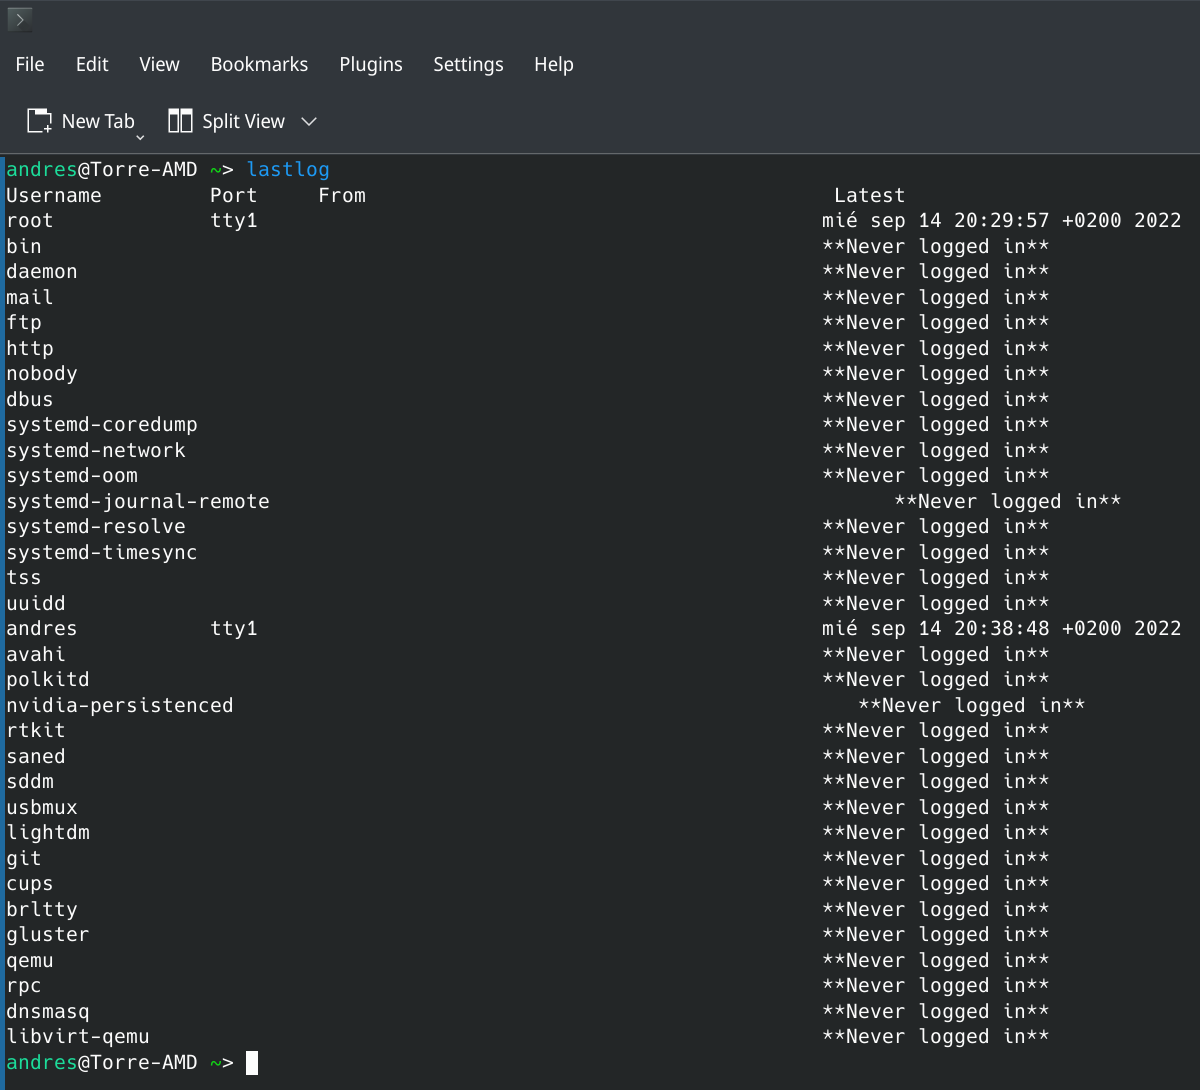
\includegraphics[width=\textwidth]{imagenes/lastlogcasa.png}
\end{figure}

COmo se puede ver, no hay ninguno en el que aparezca ssh y los inicios de sesion me concuerdan, lo cual me puede indicar que el sistema no ha sido (a simple vista) comprometido.
\subsection{PC de prácticas (máquina virtual)}
Voy a usar los mismo comandoos para la maquina virtual y comprobar su seguridad. Para suponer que el sistema ha sido comprometido, he usado SSH desde el ordenador de mi casa (host) hacia la maquina virtual.

\begin{figure}[H]
    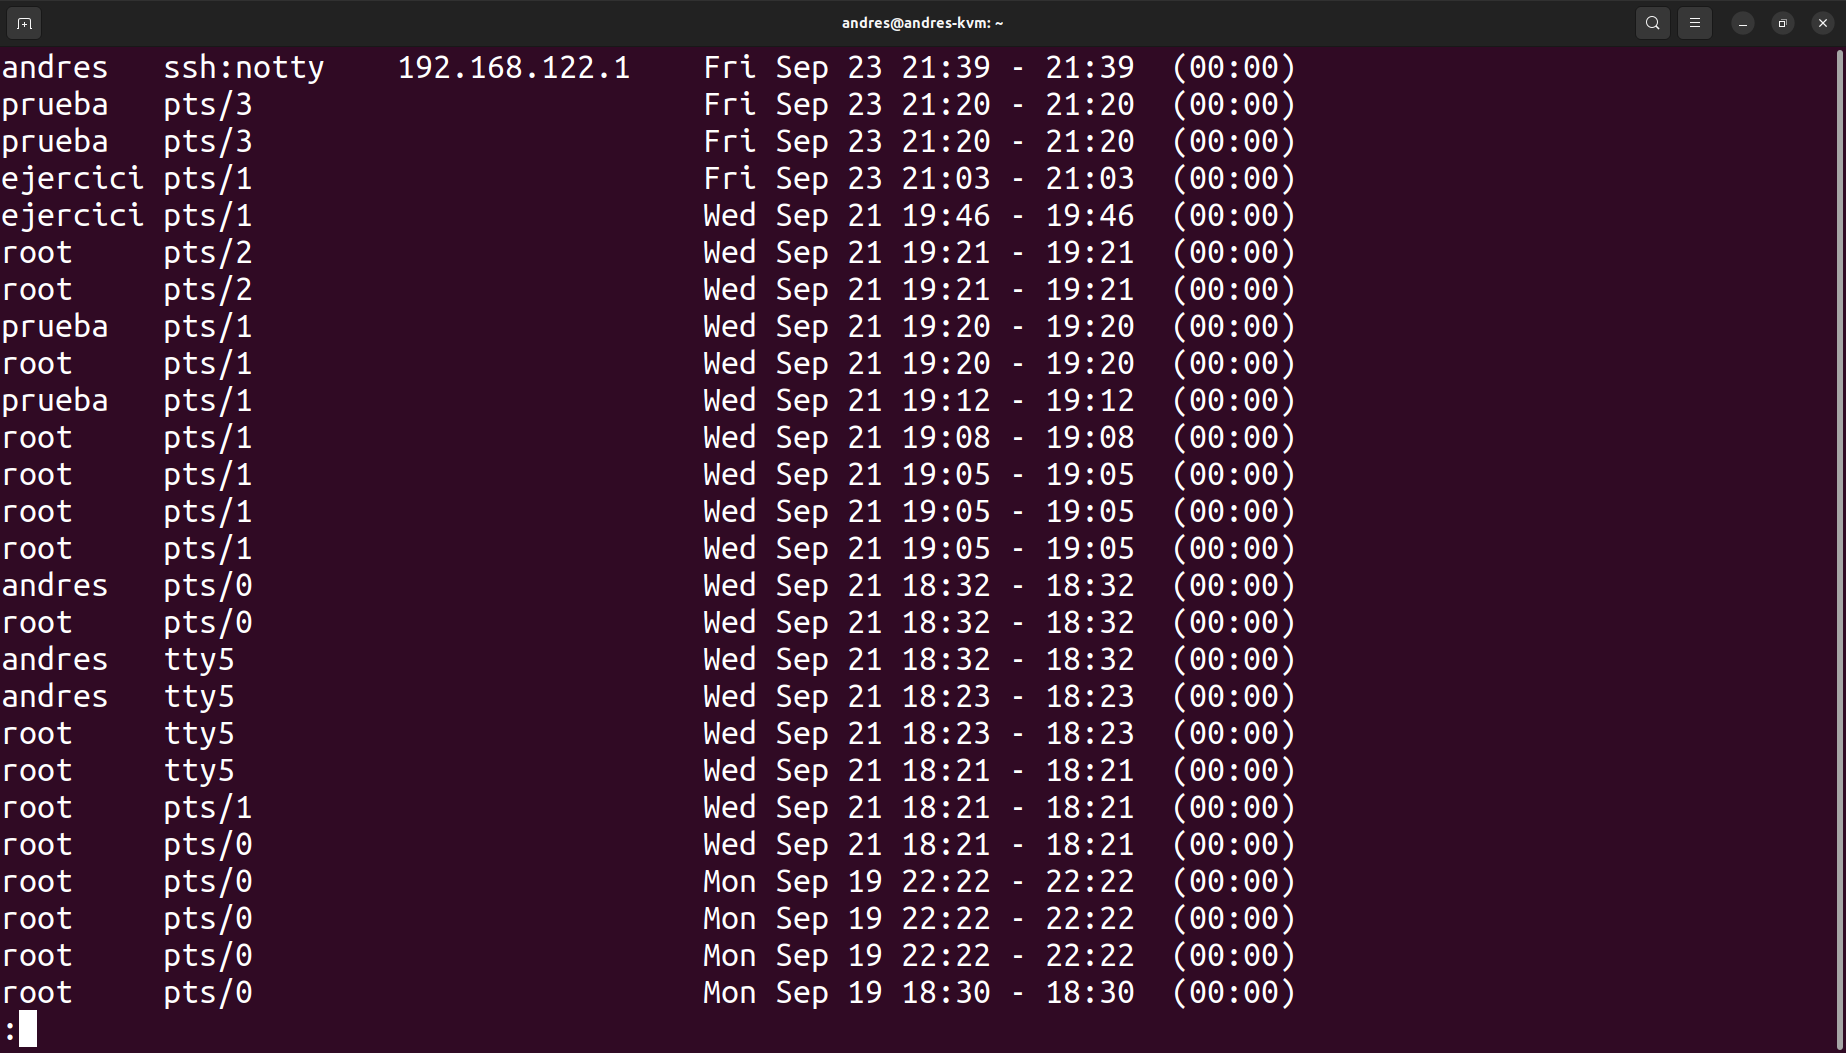
\includegraphics[width=\textwidth]{imagenes/lastbip.png}
\end{figure}

COmo se puede ver, la direccion IP ``192.168.122.1'' ha intentado conectarse a la maquona con el usuario ``andres'' por SSH. 

\begin{figure}[H]
    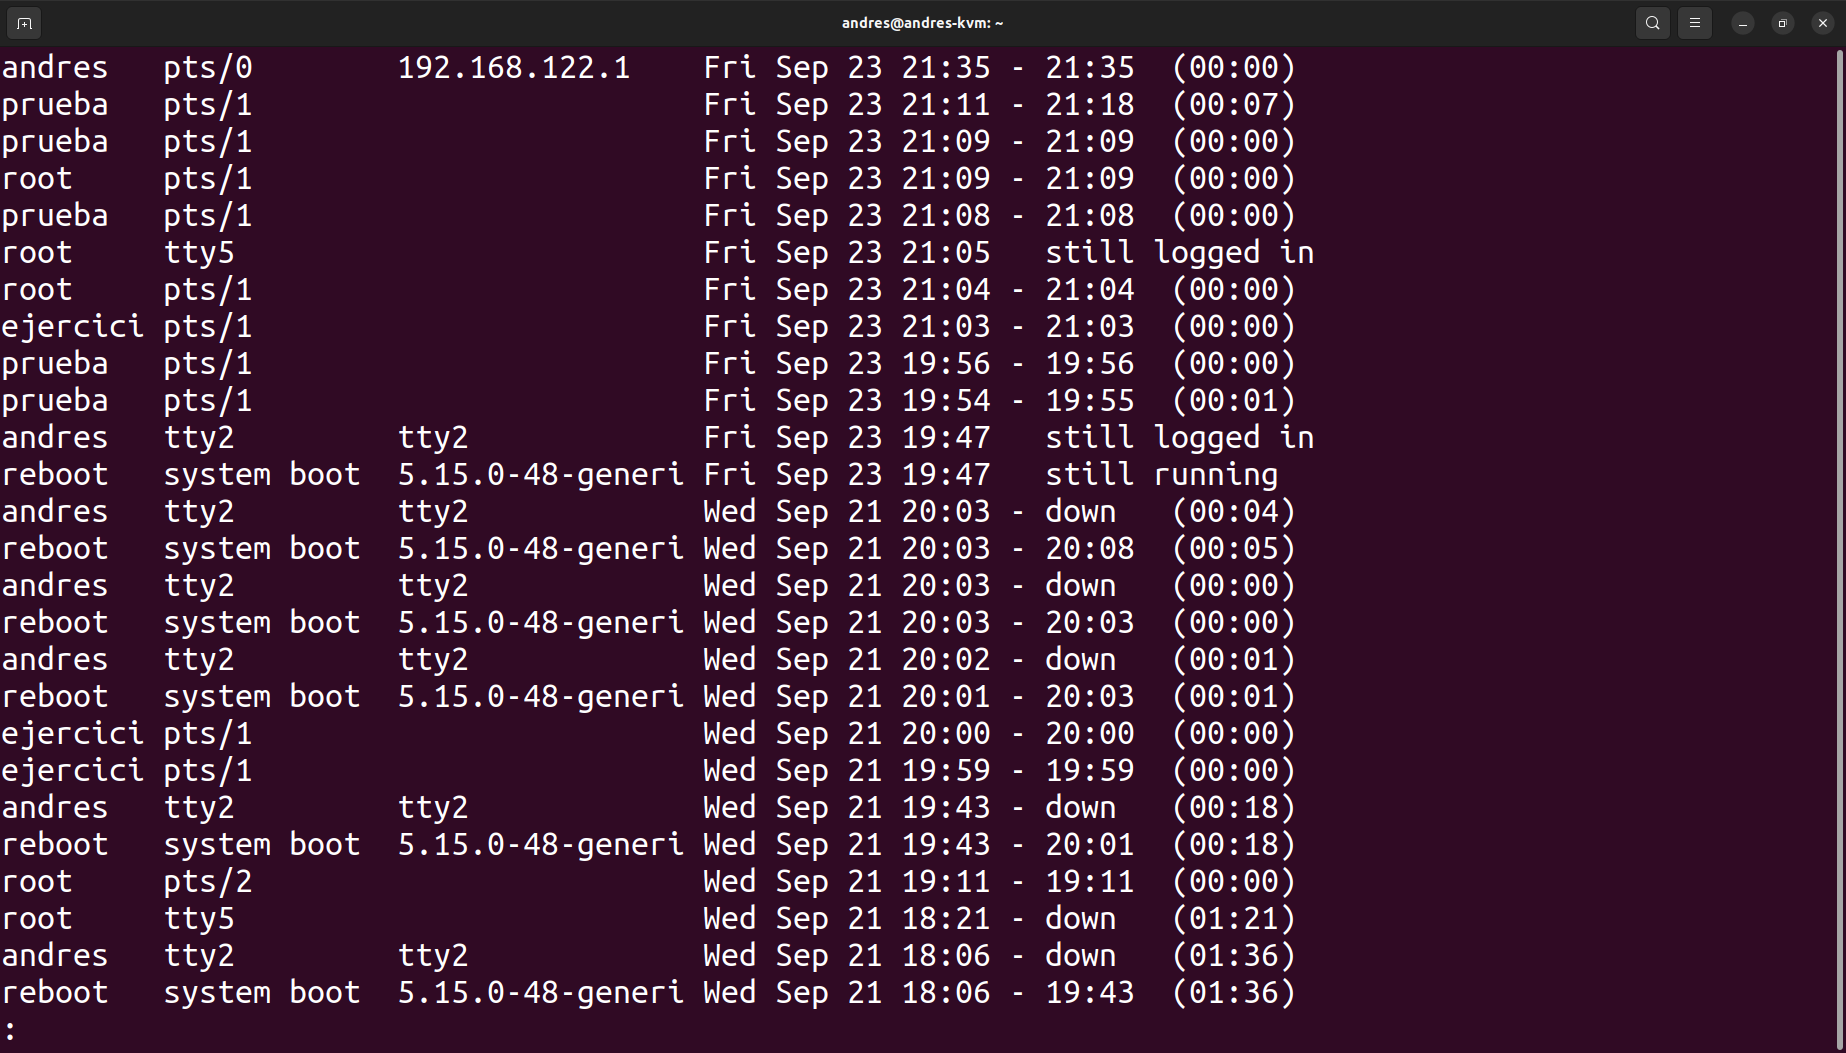
\includegraphics[width=\textwidth]{imagenes/lastip.png}
\end{figure}

Se puede observar que alguien ha entrado al sistema con SSH usando el usuario ``andres''.

\begin{figure}[H]
    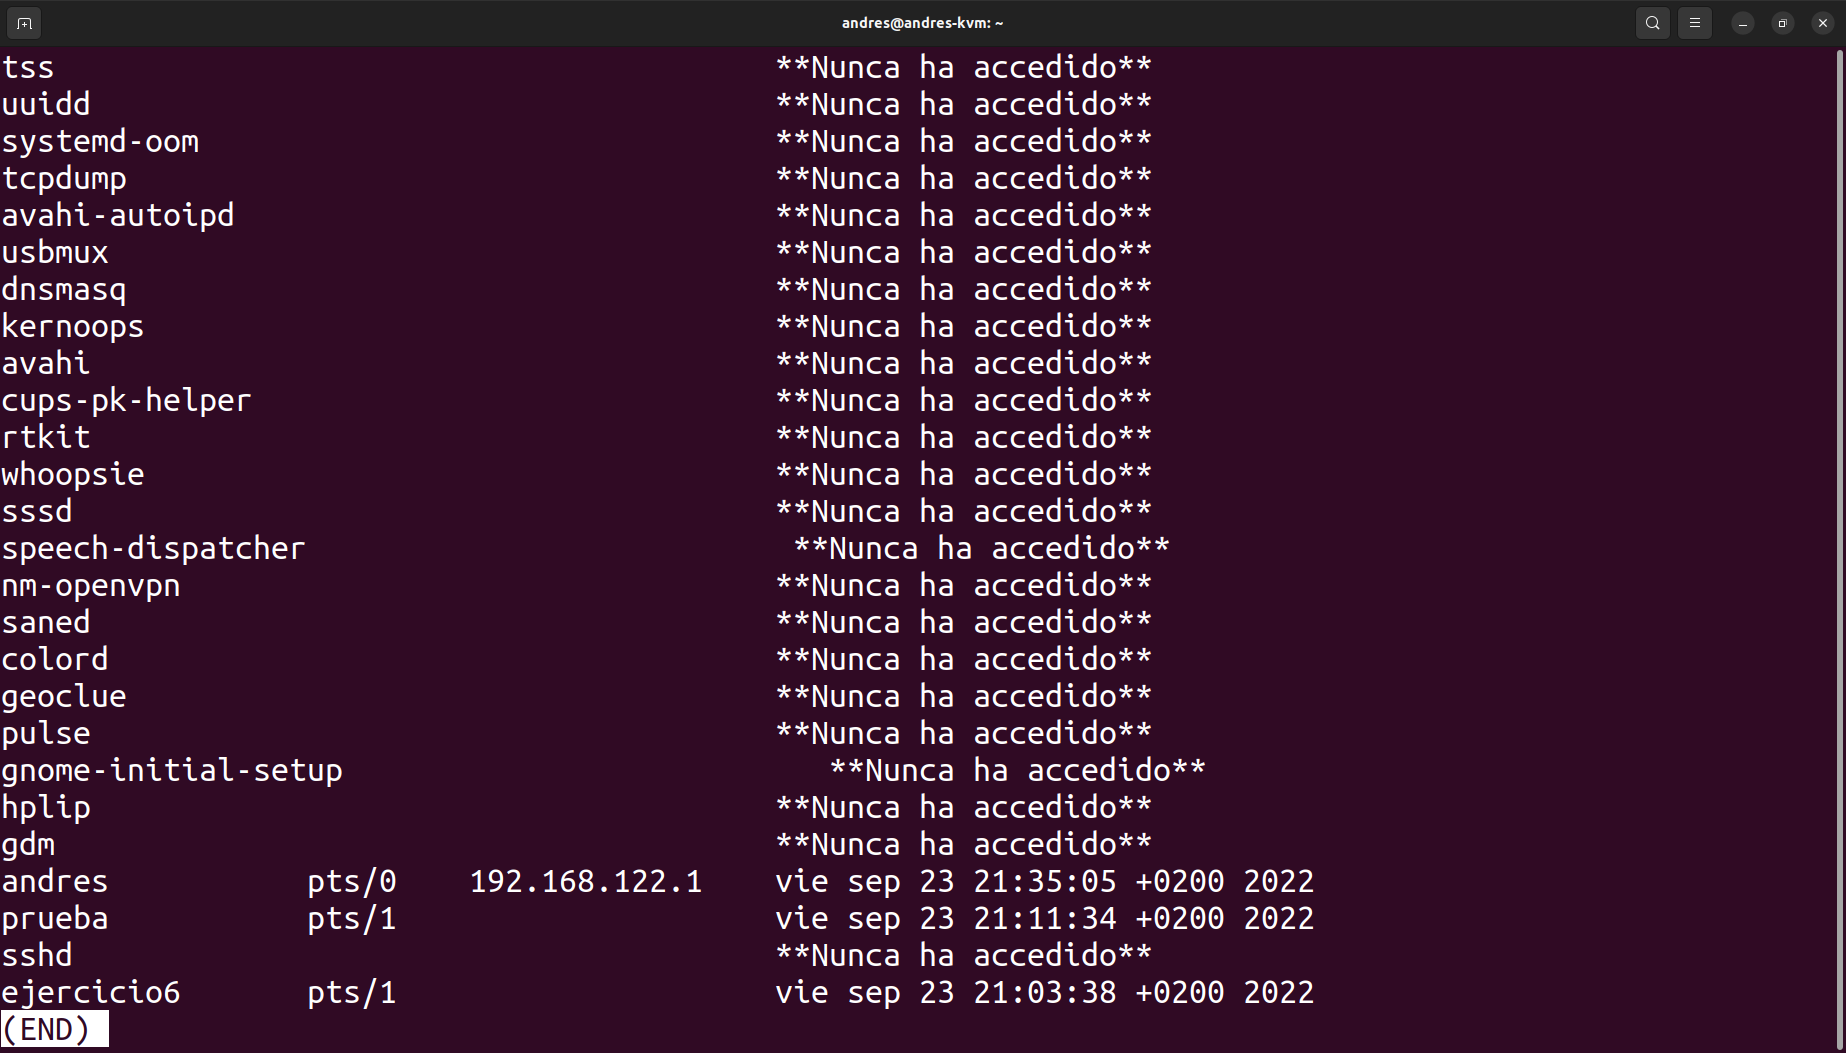
\includegraphics[width=\textwidth]{imagenes/lastlogip.png}
\end{figure}

Aqui tambien se puede observar que alguien ha accedido con la misma direccion IP anterior mediante SSH y ha conseguido iniciar sesion en el sistema.

Segun estos datos, suponiendo que no hubiera sido yo, se podria decir que alguien ha intentado acceder al sistema y ha conseguido iniciar sesion como el usuario ``andres''. Una vez sacada esta conclusion, lo recomendable es detectar los cambios que ha realizado en el sistema y el tradico de red para ver que posibles datos se ha podido llevar.
\end{document}
